\documentclass[output=paper,hidelinks]{langscibook}
\ChapterDOI{10.5281/zenodo.13347656}
\title{High vowel fricativization in Northern W\'{u} Chinese and its neighbors}

\author{Matthew Faytak\affiliation{ University at Buffalo}}

\abstract{This chapter offers a critique of strict adaptionist approaches to language change. The goal of this chapter is to discuss the possibility that an intracategorical sound change, a shift in the typical phonetic implementation of some phonological category, might unambiguously reduce the fitness of the category at issue in some sense, such that we might declare it \textit{maladaptive}. I argue that \textsc{high vowel fricativization} (HVF) is a strong candidate for just such a sound change, mainly due to the nature of the \textsc{fricative vowels} that it produces. After confirming the nature of the contrast between fricative vowels and high front vowels in a representative Northern Wú dialect\il{Northern Wú Chinese}, \SC{}\il{Sūzhōu Chinese}, with an ultrasound tongue imaging study, I present evidence that HVF introduces a relative reduction in fitness for the affected vowels in the Northern Wú context.

This reduction in fitness, which can mainly be attributed to the phonologization of a fricative noise source in fricative vowels, is not found to be balanced by some larger functional improvement, although a social function of HVF cannot be ruled out.}

\IfFileExists{../localcommands.tex}{
  \addbibresource{../localbibliography.bib}
  \usepackage{tabularx,multicol}
\usepackage{url}
\urlstyle{same}

\usepackage{listings}
\lstset{basicstyle=\ttfamily,tabsize=2,breaklines=true}

\usepackage{langsci-optional}
\usepackage{langsci-lgr}
\usepackage{langsci-gb4e}
% \usepackage{langsci-textipa}

\usepackage{csquotes}
\usepackage{multirow}
\usepackage{colortbl}
\usepackage{ulem}
\usepackage{graphicx}
\usepackage{amsmath}
\usepackage{nicefrac}
\usepackage{tabto}
\usepackage{subcaption}
\usepackage{enumitem}
\usepackage{subcaption}


\usepackage{siunitx}
\sisetup{detect-weight=true, detect-family=true, detect-all, input-symbols={\%}, free-standing-units,group-digits=false,detect-inline-weight=math}

\usepackage[linguistics, edges]{forest}
\usetikzlibrary{matrix, arrows, arrows.meta}

\usepackage{pgfplots}
\usepgfplotslibrary{colorbrewer}
\pgfplotsset{cycle list/Dark2-4}

\usepackage{derivative}
\usepackage{langsci-branding}

  
\AtBeginDocument{%
  \SetupAffiliations{output in groups = false, 
                     separator between two = {\bigskip\\},
                     separator between multiple = {\bigskip\\},
                     separator between final two = {\bigskip\\}
                   }%
}

\newfontfamily\cjkfont
  [Scale=MatchLowercase]{SourceHanSerifSC-Regular.otf}
\AdditionalFontImprint{Source Han Serif}

\newcommand{\SC}{S\=uzh\=ou Chinese}
\newcommand{\MC}{Standard Chinese}
\newcommand{\THW}{T\`{a}ih\'{u} W\'{u}}
\newcommand{\SH}{Sh\`{a}ngh\v{a}i}
\newcommand{\iz}{ɨ̻}
\newcommand{\yz}{ʉ̻}
\newcommand{\zz}{ɿ}
\newcommand{\zw}{ʮ}
\newcommand{\pri}{*\textit{i}}
\newcommand{\pry}{*\textit{y}}
\newcommand{\prien}{*\textit{jen}}
\newcommand{\pryen}{*\textit{ɥɤn}}

\newcommand{\spr}[1]{\textsuperscript{#1}}

\renewcommand{\NG}{ŋ}
\newcommand{\textsubarch}{̯}
\renewcommand{\textschwa}{ə}
\renewcommand{\textprimstress}{ˈ}
\renewcommand{\textltailn}{ɲ}

\renewcommand{\textbabygamma}{\textramshorns}
\newcommand{\textramshorns}{ɤ}
\renewcommand{\textbardotlessj}{ɟ}
\renewcommand{\textbari}{ɨ}
\renewcommand{\textbeta}{β}
\renewcommand{\textctc}{ɕ}
\renewcommand{\textdyoghlig}{ʤ}
\newcommand{\textepsilon}{ɛ}
\renewcommand{\textesh}{ʃ}
\renewcommand{\textfishhookr}{ɾ}
\renewcommand{\textglotstop}{ʔ}
\renewcommand{\textlengthmark}{}
\renewcommand{\textopeno}{ɔ}
\newcommand{\textphi}{ɸ}
\renewcommand{\textrevepsilon}{ɜ}
\renewcommand{\textrtailr}{ɽ}
\renewcommand{\textrtailt}{ʈ}
\renewcommand{\textscriptg}{ɡ}
\renewcommand{\textthorn}{þ}
\renewcommand{\textturna}{ɐ}
\renewcommand{\textturnm}{ɯ}
\renewcommand{\textturnv}{ʌ}
\renewcommand{\textyogh}{ʒ}
\renewcommand{\textramshorns}{ɤ}
\renewcommand{\textbabygamma}{\textramshorns} %babygamma obsolete
\renewcommand{\textturnm}{ɯ}

\newcommand{\tone}[1]{\textsuperscript{#1}}
\newcommand{\underarch}{\textsubarch}

\newcommand{\sg}{\textsc{sg}}


\makeatletter
\let\thetitle\@title
\let\theauthor\@author
\makeatother


\newcommand{\togglepaper}[1][0]{
%   \bibliography{../localbibliography}
  \papernote{\scriptsize\normalfont
    \theauthor.
    \titleTemp ~
    To appear in:
    Dankmar W. Enke,   Larry M. Hyman,   Johanna Nichols,   Guido Seiler \&  Thilo Weber
    Language change for the worse.
    Berlin: Language Science Press. [preliminary page numbering]
  }
  \pagenumbering{roman}
  \setcounter{chapter}{#1}
  \addtocounter{chapter}{-1}
}


\newcommand{\ilit}[1]{#1\il{#1}}
  %% hyphenation points for line breaks
%% Normally, automatic hyphenation in LaTeX is very good
%% If a word is mis-hyphenated, add it to this file
%%
%% add information to TeX file before \begin{document} with:
%% %% hyphenation points for line breaks
%% Normally, automatic hyphenation in LaTeX is very good
%% If a word is mis-hyphenated, add it to this file
%%
%% add information to TeX file before \begin{document} with:
%% %% hyphenation points for line breaks
%% Normally, automatic hyphenation in LaTeX is very good
%% If a word is mis-hyphenated, add it to this file
%%
%% add information to TeX file before \begin{document} with:
%% \include{localhyphenation}
\hyphenation{
affri-ca-te
affri-ca-tes 
Scha-den
Zú-ñi-ga
Kaj-kwa-khrat-txi
}

\hyphenation{
affri-ca-te
affri-ca-tes 
Scha-den
Zú-ñi-ga
Kaj-kwa-khrat-txi
}

\hyphenation{
affri-ca-te
affri-ca-tes 
Scha-den
Zú-ñi-ga
Kaj-kwa-khrat-txi
}

  \togglepaper[2]%%chapternumber
}{}


\begin{document}
\maketitle

\section{Introduction}\label{sec:faytak:1}

In response to the strong proposition that language change always acts to improve or optimize a changing linguistic system \citep{giacalone-ramat, vennemann}, the overarching goal of this volume (as I have understood it) is to ask whether any language change can be taken to represent some worsening of the language it affects. The task at hand is essentially to ``recognize a pejoration [\ldots{}] this being the only way to invalidate the theory'' \citep[13]{vennemann}. In my view, this task can be approached more fruitfully in an explicitly evolutionary framework, in which innovative variants in a linguistic system are successful inasmuch as they are well-adapted for communicative purposes \citep{wedel-exemplar, blevins-synopsis}. One might then seek out a maladaptive language change, then, on the basis of its stability and \textit{survival}, with maladaptive changes (a useful redefinition of changes \textit{for the worse}) tending to \textit{go extinct}. After elaborating these ideas in this section, I propose \textsc{high vowel fricativization} (HVF) to be a candidate for just such a language change and describe it in detail as it affects the northern dialects of \ili{Wú Chinese} and its neighbors.

\subsection{Adaptationist thinking and language change}\largerpage

Early research into language change as improvement generated much debate \citep{lass, samuels, lass-shitting}, and strong positions were taken in favor of the concept \citep{giacalone-ramat, vennemann}. I find that there are striking, and perhaps unexamined, parallels between the strongest accounts in favor of change as optimization and early research into adaptive mechanisms of biological evolution. Both could be argued to have followed a theoretical program of adaptationism at all costs: all developments of the systems being studied have, at some point in the history of both linguistics and evolutionary biology, been argued to improve fitness. In the case of biology, this is usually by way of natural selection. In linguistics, the mechanism has often been less specifically defined, but the parallels between \citegen{vennemann} position and the early adaptationist program critiqued by \citet{gould-lewontin} are still quite clear.

Particularly striking is the shared assumption that any local reduction in fitness cannot be pinned on natural selection, but rather on the need to implement local trade-offs to effect global optimization. As \citet[14]{vennemann} notes, ``[\ldots] it is impossible to optimize a language in all domains at once. There cannot be a perfect language but only languages in which certain parameters are optimized at the expense of others''. Nearly a decade before, Gould and Lewontin had criticized a similar viewpoint prevalent in evolutionary biology and noted its major fault:

\begin{quotation}
[\ldots{}] an organism cannot optimize each part without imposing expenses on others. The notion of ``trade-off'' is introduced, and organisms are interpreted as best compromises among competing demands. [\ldots{}] Any suboptimality of a part is explained as its contribution to the best possible design for the whole. \textit{The notion that suboptimality might represent anything other than the immediate work of natural selection is usually not entertained} (\citealp[585--586]{gould-lewontin}, emphasis mine).
\end{quotation}

At the core of this chapter is a reassessment of suboptimality in language change: evolutionary characterizations of language change at various levels of structure have become more frequent in recent years \citep{blevins-synopsis, croft-explaining, wedel-exemplar, mufwene}.
% It is the latter that is of interest for the present study, especially since
The role of natural selection is sometimes explicitly foregrounded in this line of linguistic research: well-adapted innovations in word forms and the substantive makeup of phonemes, for instance, are more \textit{successful} in terms of increased usage in the speech community due to their increased fitness at signalling linguistic contrast \citep[261--263]{wedel-exemplar}.

But these newer typologies of language change also give prominent roles to non-adaptive change, such as language contact in \citet{blevins-synopsis} or pruning of lines of descent in the case of \citet{wedel-exemplar}, a view much closer to mainstream evolutionary biology today. In many cases developmental structures in biology can be demonstrated to have a non-adaptive origin, such as the well-known evolutionary \textit{spandrels} that have coincidentally developed as a side effect or interaction of unrelated adaptive developments \citep{gould-lewontin, gould}.
%
I take it as uncontroversial that, likewise, not every language change is adaptive in the sense that it improves speech communication in some way. Such non-adaptive changes abound in biological systems; most biological mutations are in fact not favorable from an adaptive standpoint \citep[945--946]{orr}. Similar non-adaptive changes should also be seen in linguistic systems upon further inspection.


\subsection{Maladaptive language change}

%
It may also be possible to find evidence for another phenomenon: sound change that is not merely non-adaptive, but \textsc{maladaptive}, or causing deviation from known adaptive peaks \citep{schluter-nychka, crespi}.
%
Maladaptation is in fact discussed in the evolutionary biology literature but is under-studied relative to adaptation \citep{brady-etal}, likely owing to the difficulty of picking out true maladaptations in biological organisms. What constitutes fitness for a given trait in a given context must first be determined to evaluate the degree of adaptation or maladaptation that an innovation introduces \citep{lewontin, crespi}, and there are competing interpretations of how to evaluate this fitness \citep{hendry-gonzalez}.


One way of pinpointing a maladaptive outcome of change, in theory, is to document an innovative variant that, once it appears, tends to immediately be selected against and eliminated from the organism (or language) in question. This approach is similar to the methodology suggested in \citet{baum-larson} in that the examination is essentially phylogenetic, examining the inheritance of an innovative character over time (here, transmission of some novel linguistic variant within a lexicon and across a speaker population). In language, such a change should carry clear disadvantages for speech communication, perhaps in terms of contrast maintenance, so as to present a strong case.
%
A relatively unambiguous \textit{change for the worse} might be, as such, a change that clearly moves from a local optimum of performance (in terms of communicative efficiency) to a local non-optimum \citep{crespi}. Below, I put forward a candidate for just such a language change, on the grounds that the variant it creates is unambiguously unstable and results in a difficult-to-maintain contrast, an ecological situation that can be observed to result in relatively fast \textit{extinction} (within a language) of the new variant via sound change.

I am eschewing terms like \textit{worse} in favor of \textit{maladaptive}. The term \textit{maladaptive} not only identifies the concept at issue here with the one explored in evolutionary biology, but  also eliminates the value judgment implicitly cast by the term \textit{worse}, in that it has a more limited and precise definition related to local fitness of a novel linguistic variant within a language. Sloppily characterizing maladaptivity of particular linguistic innovations as a general worsening that characterizes the broader linguistic system may serve to perpetuate popular conceptions of some languages as ``primitive'' or poorly adapted to the modern world \citep{harlow-myth, evans-myth}. In discussing maladaptive change, it is important to remain clear-eyed about the racist foundations of evolutionary biology and linguistics (for an especially lurid example of both, see the portion of Ernst Haeckel's writings presented in \citealt{koerner}) and to be careful to avoid planting the seeds for further unscientific mischaracterizations of linguistic diversity.
%
% So, to make it explicit: one should not read this chapter and reach the conclusion that any language discussed here is maladapted as a whole, or is more maladapted than any other language.


Furthermore, no language is perfectly optimal: language has been conceptualized as a complex adaptive system \citep{gell-mann, lindblom-1995}, but no one language can be said to be perfectly adapted to speech communication. Any biological organism can be thought of as slightly maladapted in certain respects \citep{crespi}; analogously, I assume that all languages exhibit local non-optimality from time to time as a consequence of random drift being randomly amplified. The task at hand is thus not trivially demonstrating that language encompasses inefficiencies but rather, it is to highlight a linguistic change which appears to produce a variant of a linguistic feature that is less fit  than its predecessor.


\subsection{A possible maladaptive sound change: High vowel fricativization}

A typologically rare sound change occurs in \ili{Northern Wú Chinese}, spoken in central coastal China in and near Sh\`{a}ngh\v{a}i, as well as in some nearby \ili{Jianghuai} Mandarin varieties (e.g. Héféi\il{Héféi Mandarin}, Yánchéng\il{Yánchéng Mandarin}) and Southern Wú\il{Southern Wú Chinese} varieties (e.g. Jīnhuá\il{Jīnhuá Chinese}). Based on comparison among related Wú\il{Wú Chinese} varieties, reconstructible unrounded and rounded high front vowels \pri{} and \pry{} have come to exhibit fricative noise resembling that of a [ʑ] across much of Northern Wú\il{Northern Wú Chinese}, with the latter reflex also retaining its lip rounding.
Given the spectral properties of the frication in these segments and the fact that they are fully and modally voiced, the fricative noise cannot be attributed to non-modal phonation or devoicing, but is more readily attributable to the postalveolar constriction thought to characterize both sounds \citep[43--50]{ling, ling-phd}.
%
As such, I transcribe these \textsc{fricative vowels} throughout as /\iz{}/ and /\yz{}/, respectively.\footnote{These ad hoc transcriptions use the IPA's laminal subscript diacritic, in an extension of its typical use on coronal consonants.}
%  \citep[235]{pullum-ladusaw}
%
These two vowels typically contrast phonemically with each other and with the high front vowels /i/ and /y/, which in modern Wú\il{Wú Chinese} dialects are usually developments of lower, diphthongized, or nasalized rhymes \prien{} and \pryen{} (see \sectref{history-section} for further details).


There is reason to label this sound change, which I will refer to as \textsc{high vowel fricativization} (HVF), as maladaptive.
%
The fricative vowels which result from HVF could be argued to be less well-adapted to speech communication than their reconstructible starting states. Under HVF, high front vowels, which are noted for the stability of their motor-articulatory and articulatory-acoustic mappings \citep{fujimura-kakita, stevens-nature}, become fricative vowels, which are more aerodynamically fickle and demanding of high articulatory precision \citep{ohala83}; they are accordingly especially prone to merging with acoustically similar vowels.
%
It is difficult to find a motivation in phonetic substance for HVF in the \SC{}\il{Sūzhōu Chinese} case: based on comparison with neighboring dialects, HVF does not appear to contribute to maintenance of contrasts between the reflexes of \pri{}, \pry{}, and other vowels.
%
Rather, HVF seems to have occurred by chance, with no apparent adaptive advantage conferred on the affected segments.


In \sectref{sec:faytak:2}, I present basic information on the \SC{}\il{Sūzhōu Chinese} vowels as a descriptive example; I include evidence from an ultrasound tongue imaging study which confirms that the \SC{}\il{Sūzhōu Chinese} fricative vowels differ in tongue shape from high front vowels (i.e., /i/) and are in fact more similar to postalveolar fricatives in tongue shape (i.e., /ɕ/).
%
Following \sectref{sec:faytak:3}, which outlines a historical-comparative account of how HVF has proceeded in Northern Wú\il{Northern Wú Chinese} and other geographically adjacent Wú\il{Wú Chinese} and \ili{Mandarin} groupings, in \sectref{sec:faytak:4} I provide several arguments from phonetic substance for viewing HVF in this geographical area as a maladaptive change.
%
In \sectref{sec:faytak:5}, I speculate on the possible role of language contact in triggering HVF, but note that any social advantage that HVF confers on speakers is offset by the apparent reduction of fitness of speech sounds affected by HVF in communication.
%
I conclude by considering the implications of maladaptive change for adaptationist theories of sound change.


\section{High vowel fricativization in Northern Wú}\label{sec:faytak:2}

The present study examines \textit{high vowel fricativization} (HVF) in \ili{Northern Wú Chinese}.
%
I use the variety of \SC{}\il{Sūzhōu Chinese} to exemplify the results of the change in detail. \SC{}\il{Sūzhōu Chinese} here refers specifically to the variety of \ili{Wú Chinese} spoken in the urban core of the city of S\={u}zh\={o}u\il{Sūzhōu Chinese} {\cjkfont 苏州} and its immediate surroundings (Figure \ref{fig:wu-map}); the specific variety at issue is spoken in and around the district containing the old city (G\=us\=u q\=u {\cjkfont 姑苏区}). Below, I provide some relevant details on the vowel system of \SC{}\il{Sūzhōu Chinese} in \sectref{sec:faytak:2.1}, followed by a discussion of HVF in \SC{}\il{Sūzhōu Chinese} and neighboring Wú\il{Wú Chinese} dialects in \sectref{sec:faytak:2.2}.
%
%Discussion of HVF in \SC{} and neighboring Northern Wú\il{Northern Wú Chinese} dialects, a subgroup of Wú\il{Wú Chinese} collectively known as \THW{}\il{Tàihú Wú Chinese} 太湖吴, follows in Section 3.

\begin{figure}[t]
\caption{The Wú Chinese area (red) \citep{yan-min, yan-population, zhao-anhui}, and the location of Sūzhōu within it (shaded, right). Map derived from \protect\url{https://commons.wikimedia.org/wiki/File:China_County-level.png} under the image's CC BY-SA 3.0 license.}
% by Wikimedia Commons user ASDFGHJ, under the image's CC BY-SA 3.0 license (see \protect\url{https://creativecommons.org/licenses/by-sa/3.0/legalcode})
\label{fig:wu-map}
	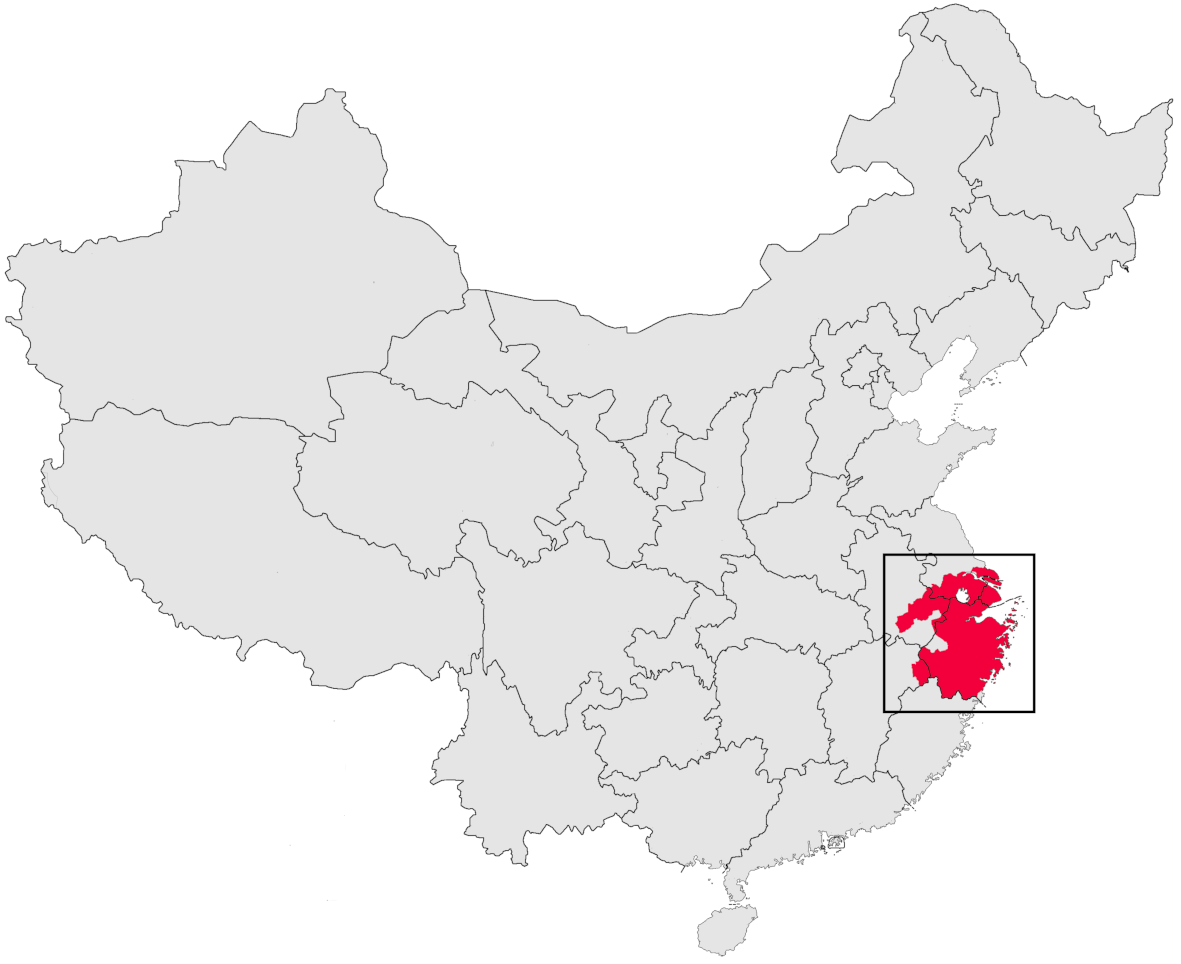
\includegraphics[height=.4\textwidth]{figures/wu-national}
	\fbox{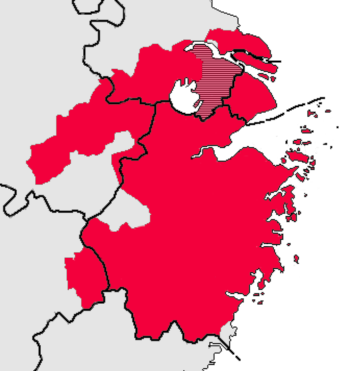
\includegraphics[height=.3\textwidth]{figures/wu-region}}
\end{figure}
\il{Wú Chinese}

\subsection{\SC{} apical and fricative vowels} \label{sec:suzhou-vowels} \label{sec:faytak:2.1}

The vowel inventory of \SC{}\il{Sūzhōu Chinese}, given in \tabref{tab:sc-inventory}, is noteworthy for including two \textsc{fricative vowels} and two \textsc{apical vowels} \citep{ling-phd, wang-suzhou}. As described below, both sets of vowels are produced with a coronal constriction, which is particularly unusual given that a dorsal constriction location is typical of the lingual articulation of most attested vowels \citep{lindblom-sundberg, lindau-vowel, honda96}. Some articulatory and acoustic characteristics of these two vowel types in \SC{}\il{Sūzhōu Chinese} and other languages further afield are discussed in this section.
%the main differences are in constriction location and phonotactics.


\begin{table}[t]
\caption{The vowel phonemes of Sūzhōu Chinese, after \citet{wang-suzhou-re, wang-suzhou} and \citet{ling-phd}. The four glottalized vowels are treated as separate phonemes, as in \citet{chen-shanghai} on Shanghainese. Vowel qualities not phonemic on distributional grounds are given in square brackets [].}
\label{tab:sc-inventory}
\begin{tabular}{c c c c c c}
\lsptoprule
 & & Unrounded & Rounded \\
\cmidrule{3-4}
\multirow{2}{*}{Coronal} & Anterior (``apical'') & \zz & [\zw] \\
 & Posterior (``fricative'') & \iz & \yz \\
\midrule
 & & \multicolumn{2}{c}{Front} & \multirow{2}{*}{Central} & \multirow{2}{*}{Back} \\
 & & Unrounded & Rounded & & \\
\midrule
\multirow{3}{*}{Dorsal} & ~~~~High ~~~ & i & y & & \\
 & ~~~Mid ~~~& ɛ & \o & ə əʔ & o oʔ\\
 & ~~~Low ~~~& a aʔ & & & ɑ ɑʔ \\
\midrule
\multicolumn{6}{c}{Other: Diphthongs əu, eɪ $\sim$ \o{}ʏ; Labial [ɯ\textsuperscript{v}], [ɯ\textsuperscript{β}] }\\
\lspbottomrule
\end{tabular}
\end{table}
\il{Sūzhōu Chinese}\il{Shanghainese}

The focus here is on the fricative vowels, which are phonotactically less restricted than the apical vowels and are described as typically exhibiting a posterior coronal (i.e., postalveolar) constriction. Some disambiguation of the apical vowels and the fricative vowels is in order.
%
Apical vowels (sh\'eji\={a}n yu\'any\={\i}n {\cjkfont 舌尖元音}) occur in Standard \ili{Chinese} \citep{leekim-s, faytak-icphs}, and they are broadly attested throughout the \ili{Chinese} languages \citep{zee-icphs, lee-encyclopedia}, including all of \ili{Wú Chinese} \citep{qian}. Apical vowels have characteristic phonotactic restrictions: they must occur following a fricative or affricate consonant that shares their place of articulation. Because of this pattern and the fact that they are most often allophones of high front vowel phonemes such as /i/, they are generally presumed to have arisen from high front vowels via coarticulation with their onsets \citep{chen-middle, yu-aero}. In \SC{}\il{Sūzhōu Chinese}, the unrounded and rounded apical vowels /\zz{}/ and [\zw{}] have the characteristic phonotactics of apical vowels,  occurring only after apico-alveolar fricative and affricate onsets (/s/, /ts/, etc.). Unlike in Standard \ili{Chinese}, on distributional grounds, the \SC{}\il{Sūzhōu Chinese} unrounded apical vowel is phonemic (see Table \ref{tab:sc-contrasts}). The \SC{}\il{Sūzhōu Chinese} vowels are described as having an apico-alveolar constriction \citep{ling-phd, wang-suzhou}, similar to the Standard \ili{Chinese} apical vowel [\zz{}] that occurs following apico-alveolar fricative and affricate onsets (/s/, /ts/, etc.).

The fricative vowels (m\'{o}c\={a}hu\`{a} yu\'{a}ny\={\i}n {\cjkfont 摩擦化元音}) in \SC{}\il{Sūzhōu Chinese} exhibit a different, more posterior constriction location compared to the apical vowels. \citep[43--50]{ling, ling-phd} identifies this constriction location as lamino-postalveolar, resembling \SC{}'s\il{Sūzhōu Chinese} lamino-postalveolar fricative consonants, e.g. /ɕ/. On the basis of Ling's data, I transcribe these two vowels as laminal /\iz{}/ and /\yz{}/. In both \SC{}\il{Sūzhōu Chinese} and in other \ili{Chinese} varieties that have them \citep{zhu-high}, fricative vowels are phonotactically less restricted than apical vowels, and may occur not only with homorganic fricative and affricate onsets (/ɕ/, /tɕ/, etc.) but also with bilabial and labiodental onsets (as is the case for /\iz{}/) or without any onset (as for /\iz{}/ and /\yz{}/). Fricative vowels such as they occur in \SC{}\il{Sūzhōu Chinese}, then, appear to arise not through assimilation to onset consonants (as is the case with apical vowels); the process of high vowel fricativization that does appear to give rise to them is explored in the next section. All \SC{}\il{Sūzhōu Chinese} fricative and apical vowels phonemically contrast with one another, except perhaps [\zw{}], which in distributional terms could be considered an allophone of /\yz{}/ (Figure \ref{tab:sc-contrasts}).

Apical and fricative vowels are attested throughout non-Standard varieties of \ili{Chinese} \citep{zhu-high, zee-icphs} and in various languages beyond the \ili{Chinese} linguistic area \citep{bjorsten1999, connell, westerberg}, notably \ili{Swedish}. The acoustic characteristic uniting the various descriptions of these segments is the consistent presence of voiced fricative noise, which appears to form part of the segments' production goals in the case of the fricative vowels. In the case of apical vowels, which obligatorily follow strident fricative or affricate onset consonants, the presence of fricative noise is perhaps unsurprising;\footnote{See \citet{leekim-s} on Standard \ili{Chinese} apical vowels as an apparent counterexample to this generalization: although they exhibit fricative-like tongue shapes and immediately follow fricative onsets, they do not appear to exhibit fricative noise consistently.} for fricative vowels, more interestingly, the affiliation of the fricative noise appears to be to the vowel itself.\largerpage[2]

Both fricative and apical vowels also exhibit a clear formant structure resembling a high central vowel, ``rather than [the] schwa-like quality often associated with syllabic fricatives'' \citep[15]{connell}. For both of the \SC{}\il{Sūzhōu Chinese} fricative vowels and the comparable unrounded vowel in dialectal \ili{Swedish}, F1 is somewhat higher, and F2 lower, than a comparable high front vowel with the same lip rounding \citep{bjorsten1999, ling-phd, schotz-i, westerberg}; apical vowels tend to have an even lower F2 than fricative vowels with the same lip rounding \citep[46--53]{ling-phd}. Both the characteristic fricative noise at high frequencies and the typical formant frequencies described here can be seen in the example spectrograms of the \SC{}\il{Sūzhōu Chinese} apical and fricative vowels in Figure \ref{tab:sc-contrasts}.
% \citet{ling-phd} posits that the decreasing F1 frequency within a rounding series in \SC{} is due to the [increasingly anterior constriction location], [which drives down F1 due to cavity affiliation swaps].

\begin{figure}[t]
\caption{Spectrograms for minimal sets of \SC{} high front vowels /i/, /y/, fricative vowels /\iz/, /\yz/, and apical vowels /\zz/, [\zw]. Examples extracted from a frame sentence with segmental context [ta \underline{\hspace{0.5cm}} kɛ].}
\label{tab:sc-contrasts}
	\setlength\tabcolsep{0pt}
	\begin{tabular}{l l l}
	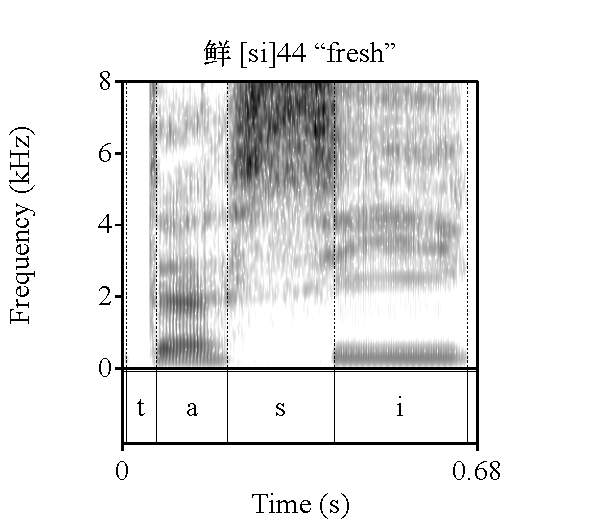
\includegraphics[trim= 0.1cm 0cm 1.25cm 0.5cm, clip=true, height=.33\textwidth]{figures/siy.pdf} &
	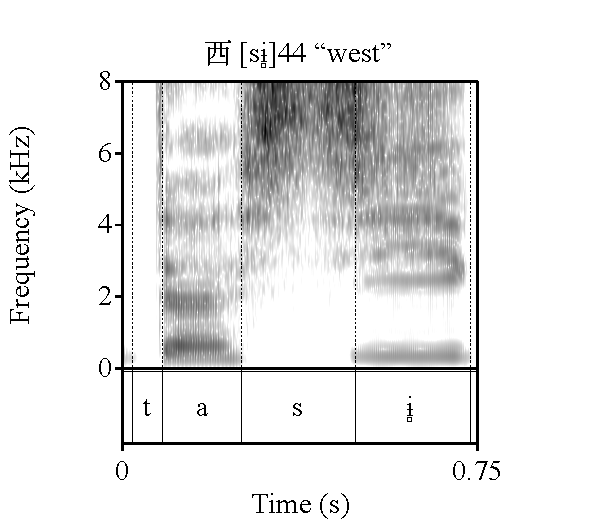
\includegraphics[trim= 1.65cm 0cm 1.25cm 0.5cm, clip=true, height=.33\textwidth]{figures/siz.pdf} &
	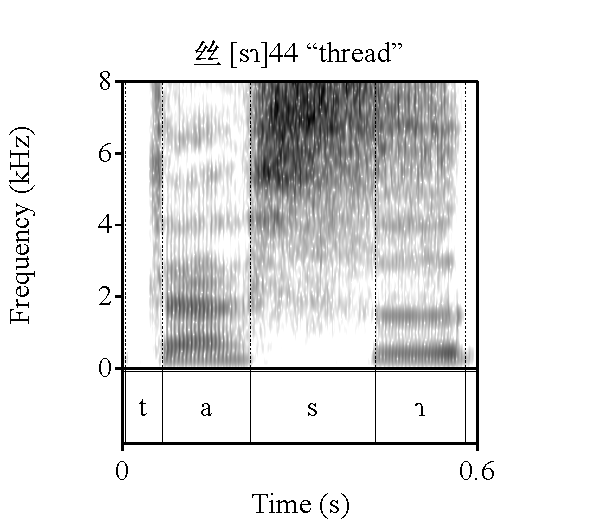
\includegraphics[trim= 1.55cm 0cm 1.25cm 0.5cm, clip=true, height=.33\textwidth]{figures/szz.pdf} \\
	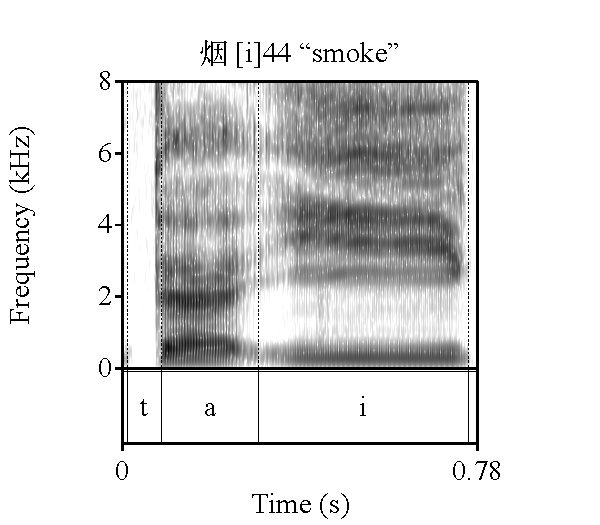
\includegraphics[trim= 0.1cm 0cm 1.25cm 0.5cm, clip=true, height=.33\textwidth]{figures/iy.pdf} &
	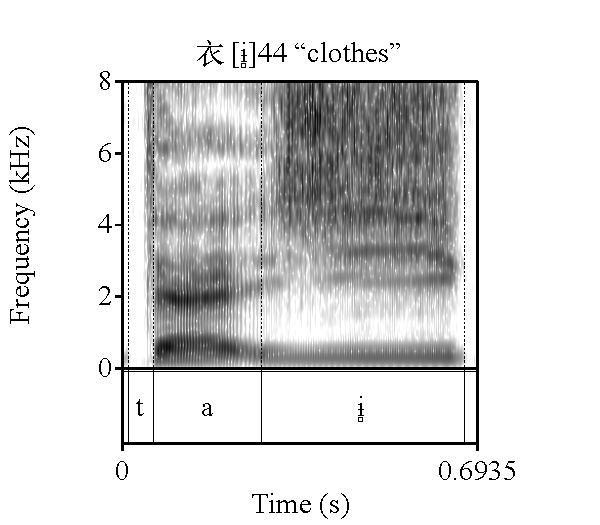
\includegraphics[trim= 1.65cm 0cm 1.25cm 0.5cm, clip=true, height=.33\textwidth]{figures/iz.pdf} &
	~
	 \\
	 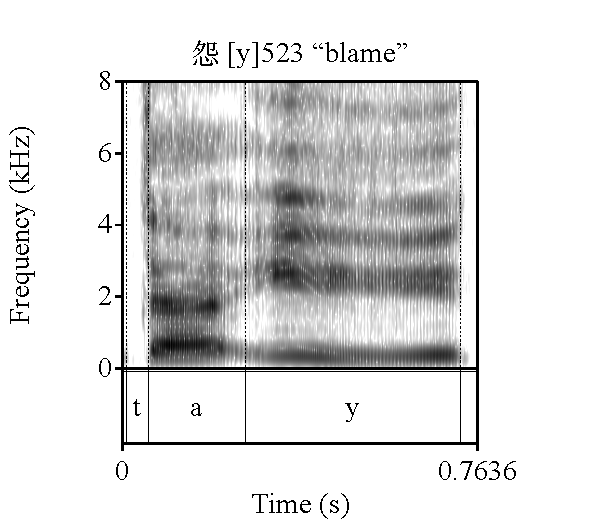
\includegraphics[trim= 0.1cm 0cm 1.25cm 0.5cm, clip=true, height=.33\textwidth]{figures/yy.pdf} &
	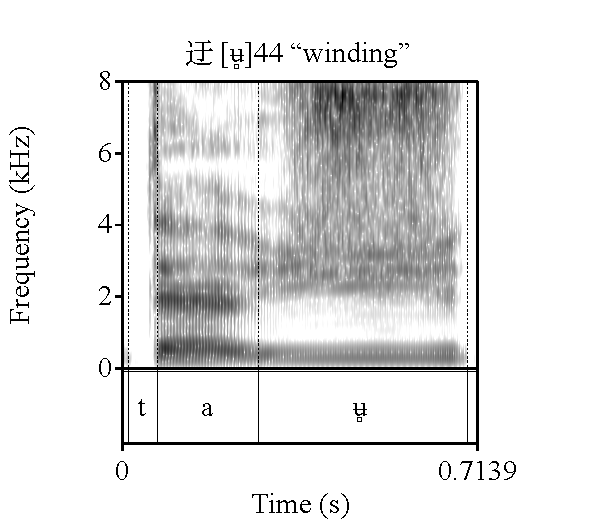
\includegraphics[trim= 1.65cm 0cm 1.25cm 0.5cm, clip=true, height=.33\textwidth]{figures/yz.pdf} &
	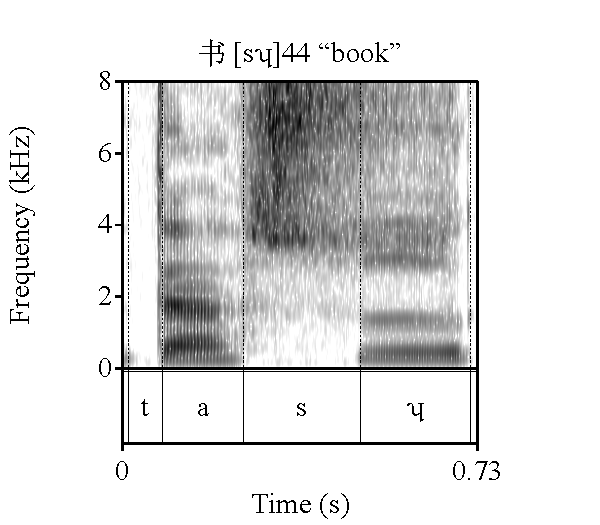
\includegraphics[trim= 1.55cm 0cm 1.25cm 0.5cm, clip=true, height=.33\textwidth]{figures/szw.pdf} \\
	\end{tabular}
\end{figure}
\il{Sūzhōu Chinese}

The fricative noise associated with both apical and fricative vowels is typically strident in quality \citep{rose-diss, bjorsten1999, connell, ling-phd}, suggesting that the tongue is configured to direct a turbulent jet of air at the alveolar ridge or teeth, but the specific quality and intensity of the resulting frication varies somewhat among speakers. Other plausible sources of fricative noise can be ruled out. Some dialects of \ili{Wú Chinese} are known for their register systems involving contrastive use of breathiness or other non-modal phonation \citep[323]{rose-yang, cao-maddieson, chen-gussenhoven}. The fricative noise in apical and fricative vowels does not appear to be a manifestation of a register contrast in Northern Wú\il{Northern Wú Chinese}, including \SC{}\il{Sūzhōu Chinese}. Fricative and apical vowels are characterized by uninterrupted modal voice, and the non-laryngeal character of their fricative noise is evident from its spectral shape, visible in Figure \ref{tab:sc-contrasts} above 4kHz,\largerpage{} in a reasonable range for sibilant or shibilant fricatives. The common element across speakers is the production of some type of fricative noise with a supralaryngeal constriction, most often coronal.\footnote{An anonymous reviewer points out that all of the languages mentioned in this section are tonal in some sense. We reserve further comment on the connection between tonality and HVF for future research: it cannot be ruled out, for instance, that some third characteristic predisposes languages to the development of both lexical tone contrasts and fricative noise contrasts on vowels.}


\subsection{The fricative vowel-high front vowel contrast: an ultrasound study} \label{ultrasound}\label{sec:faytak:2.2}

A relative abundance of data exists showing that the apical vowels are produced with a constriction made at the alveolar ridge by the tongue tip, similar to [s], in both \MC{}\il{Chinese} and \SC{}\il{Sūzhōu Chinese} \citep{zhou-wu, ling-phd, leekim-s, faytak-icphs}.
%
To confirm that the fricative vowels are articulated similarly to other fricative consonants such as [ɕ] in \SC{}\il{Sūzhōu Chinese}, data on the \SC{}\il{Sūzhōu Chinese} high front vowel /i/, the fricative vowel /\iz/, and the fricative consonant /ɕ/ were collected using ultrasound tongue imaging. Eight participants (four male, four female) were recruited at the University of California, Berkeley and were compensated for their time and effort; all procedures described here were approved by the UCB institutional review board.

Recording took place in a sound-attenuated booth in the UC Berkeley PhonLab. Participants were asked to read the monosyllabic stimuli shown in Table \ref{tab:1:stimuli} with a \SC{}\il{Sūzhōu Chinese} reading (as opposed to a \MC{}\il{Chinese} reading). Stimuli containing the target segments were displayed as simplified \ili{Chinese} characters on a computer screen. Each stimulus item was read embedded in the frame sentence given in \ref{ex:1:frame}:

\ea\label{ex:1:frame}
\let\eachwordone\cjkfont
Frame sentence \SC{}\\
\glll 我 说 \underline{\hspace{0.5cm}} 拨 你 听。 \\
	ŋəu\tone{11} səʔ\tone{33} \underline{\hspace{0.5cm}} pəʔ\tone{33} neɪ\tone{22}  tʰɪŋ\tone{33}\\
	1{\sg} say \underline{\hspace{0.5cm}} give 2{\sg} hear\\
\glt `I say \underline{\hspace{0.5cm}} to you'
\z
\il{Sūzhōu Chinese}

\noindent Readings for each stimulus item were prompted in randomized order for eight blocks. This resulted in a maximum of 48 stimuli per participant containing 64 tokens of target segments (since two words contain both /ɕ/ and a vowel: 24 tokens of /\iz{}/, 24 /i/, and 16 /ɕ/). Speakers 1 and 2 completed only five blocks of the study and so have only 40 tokens of target segments (15 /\iz{}/, 15 /i/, and 10 /ɕ/).
%
Several tokens were discarded due to recording errors; as a result, Speaker 3 has one less token of /ɕ/ and /\iz{}/ than would be expected, Speaker 4 is missing one token of /\iz{}/, Speaker 7 is missing one token of /i/, and Speaker 8 is missing one token of /ɕ/ and two tokens of /\iz{}/.

\begin{table}
\caption{Stimuli for ultrasound study; from \citet{ye-suzhou}.} \label{tab:1:stimuli}
 \begin{tabular}{lll}
  \lsptoprule
  Onset	& /\iz/ 			& /i/ 		\\
  		\midrule
  /∅/		& \cjkfont 衣 				& \cjkfont 烟 		\\
  		& \iz{}\textsuperscript{44}	& i\textsuperscript{44} \\
		& `clothes' 		& `smoke' \\
		\midrule
  /p/ 		& \cjkfont 比 		& \cjkfont 边 		\\
    		& p\iz{}\tone{5}\tone{1}	& pi\tone{44}		\\
		& `compare' & `side' \\
		\midrule
  /ɕ/ 		&\cjkfont  稀 		& \cjkfont 掀 		\\
  		& ɕ\iz{}\tone{44}	& ɕi\tone{44}		\\
		& `rare' 	& `flip' 	\\
  \lspbottomrule
 \end{tabular}
\end{table}

Ultrasound video of the resulting utterances was recorded in midsagittal section at a frame rate of 107 Hz using an Ultrasonix SonixTablet. The device was equipped with a C9-5/10 microconvex transducer held in place by an Articulate Instruments Ltd. aluminum stabilization headset, as described in \citet{headset}. Audio was recorded with an AKG 535 EB microphone and digitized through a Steinberg UR22 USB audio interface. %Recorded audio was synchronized with the ultrasound video using a synchronization signal output by the ultrasound device.
%
Frames corresponding to the acoustic midpoints of /\iz{}/, /i/, and /ɕ/ were selected using acoustic landmarks in time-aligned audio, and tongue surface contours were semiautomatically extracted using EdgeTrak \citep{edgetrak-article}. Each speaker's contours were submitted to a smoothing-spline ANOVA (SSANOVA) model to estimate the speaker's typical tongue shape for each segment \citep{gu-ssanova, davidson2006}; a polar coordinate system was used to reduce distortion in the tongue blade and root regions \citep{mielke-polar}.
%
Separately, the position of a portion of the hard palate was estimated for each speaker from the average of five frames showing maximal tongue-palate contact during a swallow task.\footnote{No palate trace is available for Speaker 3 due to their incomplete swallow task.}
%
Since individual anatomical variation cannot easily be factored out of the data, tongue shape comparisons are made within the model outputs of single speakers.

\begin{figure}[p]
\caption{Smoothing-spline ANOVA estimates of tongue contour position with 95\% confidence intervals for /\iz{}/, /i/, and /ɕ/, with palate trace (dotted line) when available. Right is anterior.}
\label{fig:2:ssanova}
	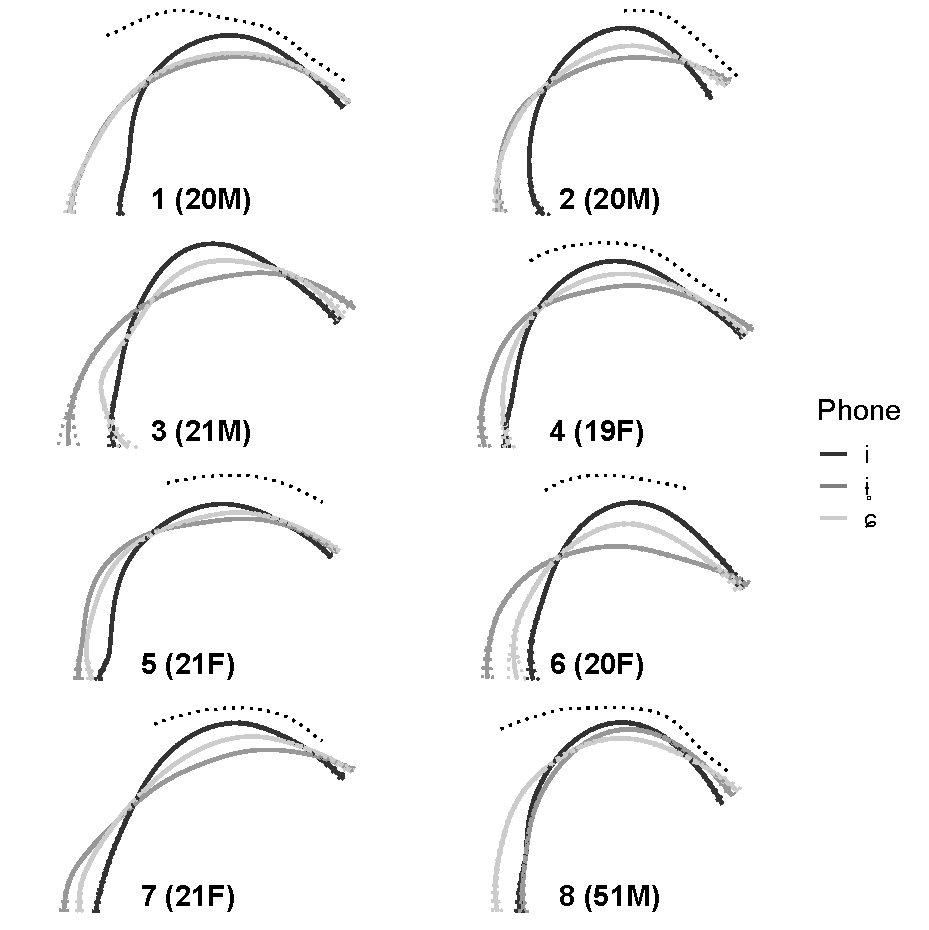
\includegraphics[width=\textwidth]{figures/SSANOVAS-2by4}
\end{figure}

SSANOVA splines are presented for each speaker in Figure \ref{fig:2:ssanova}, which shows that /\iz{}/ is more similar to /ɕ/ than /i/ across speakers: /ɕ/ and /\iz{}/ both typically exhibit a retracted tongue root, lowered tongue dorsum, and raised tongue blade in opposition to [i], which exhibits an advanced root, raised dorsum, and lowered blade.
%
Speaker 6 excepted, enough of the tongue blade is visible to directly suggest a similar postalveolar constriction for both /ɕ/ and /\iz{}/.
%
Most speakers' /\iz{}/ tongue shapes differ from those used for /ɕ/ primarily in that /ɕ/ exhibits a raised tongue dorsum relative to /\iz{}/.
%
For Speakers 1, 2, and 5, this difference is slight, but for Speakers 3, 4, 6, and 7, a greater degree of tongue dorsum raising distinguishes /ɕ/ from /\iz{}/.

\begin{figure}[t]
\caption{Smoothing-spline ANOVA estimates of tongue contour position for /ɕ/ preceding the two vowels in the data set, with 95\% confidence intervals and palate trace (dotted line) when available. Right is anterior.}
\label{fig:3:ssanova}
	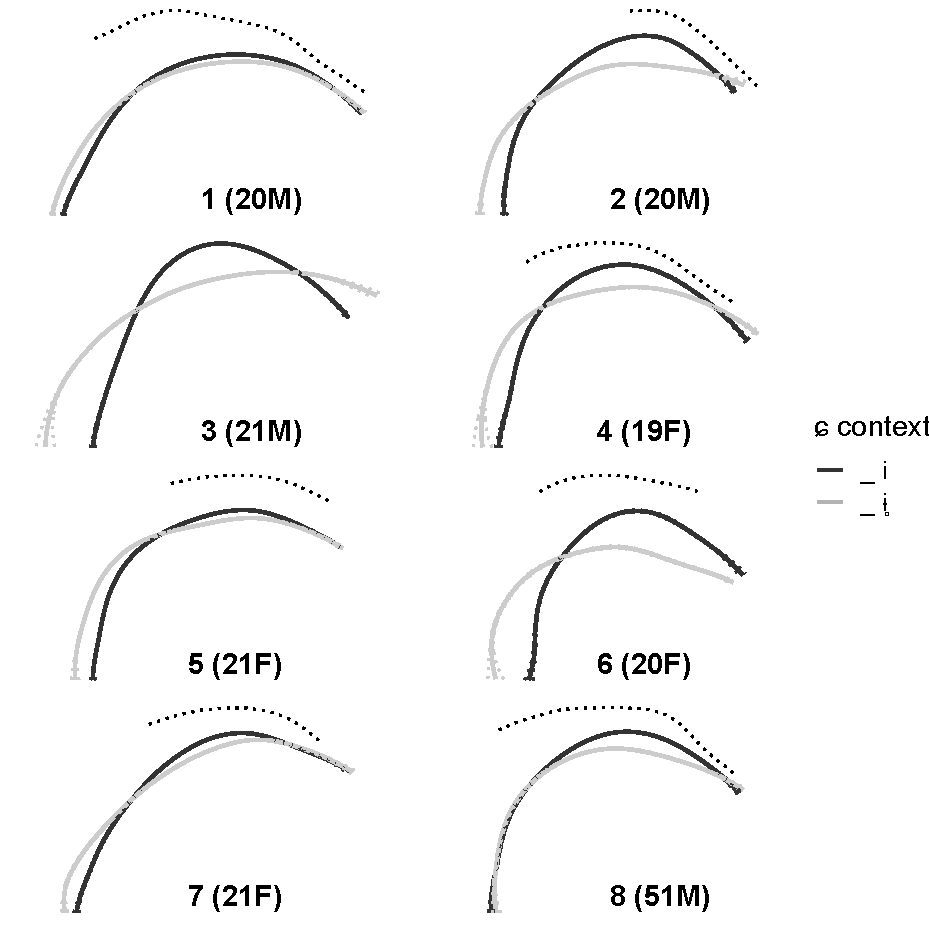
\includegraphics[width=\textwidth]{figures/SSANOVAS-SH}
\end{figure}

This inter-speaker variation in similarity between /ɕ/ and /\iz{}/ appears to be mediated by coarticulation of the onset consonant /ɕ/ with the following vowel.
%
Tokens of /ɕ/ which are followed by /i/ have a more domed tongue shape which differs substantially from /ɕ/ followed by /\iz{}/ as well as /\iz{}/ itself, a difference which can be attributed to coarticulation with /i/ (Figure \ref{fig:3:ssanova}).
%
The extent of this coarticulation in half of the /ɕ/ tokens mirrors the extent to which a speaker's /ɕ/ resembles their /\iz{}/ in terms of \textit{overall} tongue position found by the SSANOVA models shown in Figure \ref{fig:2:ssanova}.
%
Speakers 1 and 5 show the least coarticulation, which is reflected in the close overall similarity of their /ɕ/ and their /\iz{}/. Other speakers (notably Speakers 3 and 6) have more dramatic coarticulatory differences, and the overall SSANOVA result for /ɕ/ in Figure \ref{fig:2:ssanova} is a spline intermediate in shape between the two /ɕ/ variants but resembling neither.
%
% Several speakers (e.g. 3 and 4) appear to have a laminal variant of /ɕ/ before /i/, and an apical one before /\iz{}/, judging from the raising or lowering of the tongue blade.

Speaker 8 qualitatively differs from the other speakers in producing /\iz/ similarly to /ɕ/ in some respects and to /i/ in others.
%
Speaker 8's /\iz{}/ has a raised tongue blade closer in character to that of /ɕ/,  a behavior exhibited in common with the other seven speakers.
%
However, Speaker 8's /\iz{}/ is produced with an advanced tongue root and raised tongue dorsum, more akin to /i/.
%
This variant of /\iz{}/ could be described as dorso-postalveolar in articulation,  somewhat akin to an [i] articulated further front, with the tongue dorsum and blade shifted toward the postalveolar area.
%
Speaker 8 is closer in age to the population studied in \citet{ling-phd}, members of which are described as using one of two articulations for /\iz{}/: a lamino-postalveolar variant similar to the one described here for Speakers 1--7, and a dorso-postalveolar variant which resembles Speaker 8's /\iz{}/.
%
This raises the possibility that the observed difference is related to speaker age.

Regardless of speaker idiosyncrasies, and taking coarticulation of /ɕ/ with /i/ into account, the typical articulation of /\iz{}/ is much more similar to /ɕ/ than to /i/ for all speakers, especially in that a postalveolar constriction location is observed for /\iz{}/ which is absent in /i/.
%
The location of this constriction is typically quite close to the constriction for /ɕ/, which suggests an articulatory-acoustic goal shared among these segments: the production of strident fricative noise of a specific quality close to that of /ɕ/.
%
%Having established the nature of the contrast between fricative and non-fricative vowels in S\=uzh\=ou \ili{Chinese}, we move on to consdering developments in the dialect group as a whole.


\section{Diachrony of high vowel fricativization in Wú Chinese}\label{sec:faytak:3}

Having confirmed the nature of the contrast between /i/ and /\iz{}/ -- and by extension, that between /y/ and /\yz{}/ -- we turn to high vowel fricativization (HVF), the sound change that gives rise to the fricative vowels from high front vowels. The focus here is on the Northern Wú\il{Northern Wú Chinese} dialect continuum, most of which belong to the Tàihú\il{Tàihú Wú Chinese} (Lake Tài) subgroup of Wú\il{Wú Chinese} dialects. \THW{}\il{Tàihú Wú Chinese} can in turn be subdivided into the coastal S\=uh\`uji\=a {\cjkfont 苏沪嘉} group, which contains the relatively well-studied local dialects of S\=uzh\=ou\il{Sūzhōu Chinese}  and the Shàngh\v{a}i\il{Shanghainese} area\footnote{\textit{S\=uh\`uji\=a}\il{Sūhùjiā} is an initialism referring to S\=uzh\=ou {\cjkfont 苏州}, {\cjkfont 沪渎} H\`udú (an archaic name for Shàngh\v{a}i), and {\cjkfont 嘉兴} Ji\=ax\={\i}ng\il{Jiāxīng Chinese}.}, and the inland \ili{Pílíng} {\cjkfont 毗陵} group, spoken north and east of Lake Tài to the Yangtze River \citep[2--3]{qian}.
%
Southern Wú\il{Southern Wú Chinese} is phonologically conservative and with one apparent exception (Jīnhuá\il{Jīnhuá Chinese} {\cjkfont 金华} dialect; see \citealt{qian}) do not undergo HVF \citep[229]{cao-southern}. As such, they are not discussed here except as an out-group to Northern Wú\il{Northern Wú Chinese}, for instance in Table \ref{tab:hvf-2}.

After an overview of HVF in \THW{}\il{Tàihú Wú Chinese}, I begin to consider motivations for the sound change.
%
I describe the process as one of transphonologization starting in \sectref{phonologization}.
%
Two possible origins for this transphonologization are considered: one in which encroachment of the lower rhymes on the acoustic space of the higher rhymes gradually makes frication a more important cue to the latter, and one in which frication becomes an important cue essentially at random.
%
Surprisingly, the second origin is better supported by the detailed chronology of HVF and related changes to the lower rhymes in \THW{}\il{Tàihú Wú Chinese},
%
a finding which later factors in to the conclusion that HVF does not confer any clear advantage on the \THW{}\il{Tàihú Wú Chinese} high vowels.


\subsection{History and extent of HVF in Northern Wú} \label{history-section} \label{sec:faytak:3.1}

Comparative data from \ili{Wú Chinese} makes it clear that historical high front vowels are the origin of today's fricative vowels in \SC{}\il{Sūzhōu Chinese} and other closely related Wú\il{Wú Chinese} dialects. HVF has affected most of the Northern Wú\il{Northern Wú Chinese} varieties within Tàihú\il{Tàihú Wú Chinese} Wú and relatively few Wú\il{Wú Chinese} varieties beyond it to the south, although it is also observed in the less closely related Ji\={a}nghu\'{a}i\il{Jianghuai} {\cjkfont 江淮} \ili{Mandarin} dialects spoken to the north and west across the Yangtze, for instance Y\'anch\'eng\il{Yánchéng Mandarin} {\cjkfont 盐城} Mandarin \citep{cai-yancheng} and H\'ef\'ei\il{Héféi Mandarin} {\cjkfont 合肥} Mandarin \citep{hou-hefei, kong-etal}.

Wú\il{Wú Chinese}-internal comparative evidence laid out in Table \ref{tab:hvf-1} indicates that the fricative vowels are reflexes of the \ili{Proto-Wú} vowels \pri{} and \pry{}, as reconstructed in \citet{ballard}. Comparison of the \THW{}\il{Tàihú Wú Chinese} group with Wú\il{Wú Chinese} dialects further afield makes it clear that \ili{Proto-Wú} \pri{} and \pry{} were likely conventional high front vowels, given that an overall majority of reflexes for this reconstructed set are [i] or [y]. In the \THW{}\il{Tàihú Wú Chinese} varieties spoken west of Shàngh\v{a}i, exemplified here by D\=any\'ang\il{Dānyáng Chinese} and S\=uzh\=ou\il{Sūzhōu Chinese}, \citet{qian} transcribes the reflexes of the \ili{Proto-Wú} high front vowels as high front vowels with subscripted \textit{z} or \textit{j}/\textit{ʮ}. The subscripts are intended to indicate subtle differences in the quality of the frication noise produced: the former indicates that the vowel is ``accompanied by a [z] sound,'' while the latter refers to a more general ``accompanying frication'' \citep[12]{qian}. Qian's transcriptions (\textit{i$_z$}, \textit{i$_j$}, \textit{y$_z$}, etc.) can readily be identified as the fricative vowels [\iz{}] and [\yz{}] described in \sectref{sec:suzhou-vowels}.

\begin{table}
\caption{Some Tàihú Wú cognate sets that undergo HVF, from \citet{qian} with Proto-Wú reconstructions from \citet{ballard}. Vowel qualities in \SC{} are from my own notes.}
\label{tab:hvf-1}
	\begin{tabular}{l l  l l l l}
	\lsptoprule
	Proto-W\'{u} & & D\=any\'ang & S\={u}zh\={o}u & Sh\`{a}ngh\v{a}i & Tàipíng \\
	% \ili{Tàipíng} is in Sheng county, outside of Tàihú\il{Tàihú Wú Chinese} area - phonologically conservative
	\midrule
	% unrounded
	{\cjkfont 闭} {*pi\spr{III}} &  `close' & p\iz{}\spr{324} & p\iz{}\spr{412} & pi\spr{334} & pi\spr{35} \\
	{\cjkfont 移} {*ɦi\spr{I}} &  `move' & ɦ\iz{}\spr{213} & ɦ\iz{}\spr{223} & ɦi\spr{113} & ɦi\spr{312} \\
	{\cjkfont 变} {*pjen\spr{III}} &  `change' & pɪ\spr{324} & pi\spr{412}  & pi\spr{334} & pi\~e\spr{35} \\
	{\cjkfont 片} {*p'jen\spr{III}} &  `slice' & pʰɪ\spr{324} & pʰi\spr{412} & pʰi\spr{334} & pʰi\~{e}\spr{324} \\
	% rounded
	\midrule
	{\cjkfont 居} {*ky\spr{I}} &  `home' & tɕ\yz{}\spr{22} & tɕ\yz{}\spr{44} & tɕy\spr{52} & tɕy\spr{523} \\
	{\cjkfont 雨} {*ʔy\spr{II}} &  `rain' & \yz{}\spr{44} & ɦ\yz{}\spr{231} & ɦy\spr{113} & ɦy\spr{22} \\
	{\cjkfont 捐} {*kɥɤn\spr{I}} &  `donate' &	tɕʏ\spr{22} & tɕy\spr{44} & tɕy\o\spr{52} & tɕy\~{œ}\spr{523} \\
	{\cjkfont 远} {*ʔɥɤn\spr{II}}  &  `far' & ʏ\spr{44} & ɦy\spr{231} & ɦy\o\spr{113}  & ɦy\~{œ}\spr{22} \\
	\lspbottomrule
	\end{tabular}
\end{table}
\il{Tàihú Wú Chinese}\il{Proto-Wú}\il{Sūzhōu Chinese}\il{Tàipíng Chinese}\il{Dānyáng Chinese}\il{Shanghainese}

HVF as a sound change does not uniformly apply across Northern Wú\il{Northern Wú Chinese}, judging from the varied reflexes of \ili{Proto-Wú} \pri{} and \pry{}.
%
Wú\il{Wú Chinese} varieties spoken at the southern end of the Northern area do not appear to have undergone HVF for the most part. This group is represented in Table \ref{tab:hvf-1} by the Tàipíng \il{Tàipíng Chinese} variety, one of the southernmost and most phonologically conservative Northern Wú\il{Northern Wú Chinese} dialects.
%
In addition, the \SH{}-area dialects at the core of the Tàihú\il{Tàihú Wú Chinese} area do not exhibit fricative vowels at present, and in fact the reflexes of \ili{Proto-Wú} \pri{} and \pry{} are sometimes merged with the reflexes of two other \ili{Proto-Wú} rhymes, \prien{} and \pryen{}, in these varieties. In Table \ref{tab:hvf-1}, these varieties are represented by the Shàngh\v{a}i dialect of the city center.


There is evidence, however, that the \SH{}-area dialects \textit{did} undergo HVF, only to subsequently merge the unrounded fricative vowel and unrounded high front vowel and lose frication on the rounded fricative vowel.
%
Merger of reflexes of \pri{} and \prien{} is prominently mentioned in a number of descriptions of urban \ili{Shanghainese} beginning in the mid-twentieth century, starting with speakers who came of age in the 1980s \citep{xu-tang-62, xu-tang, chen-zm-diss}.
%
The unmerged reflex of \pri{} is described as fricated whenever a detailed phonetic description is included:
\citet[45]{qian} notes that some speakers still read modern \SH{} /i/ and /y/ with a fricative quality, and both \citet[14]{zhu-grammar} and \citet[329--330]{chen-gussenhoven} observe a contrast based in part on the presence or absence of frication in the reflexes of \ili{Proto-Wú} \pri{} and \prien{} for some of their older consultants.
%
HVF also seems to have affected \ili{Proto-Wú} \pry{} in \SH{}, based on Qian's comments, but the resulting fricative quality was not, on its own, the primary means of signaling contrast with some other vowel: \ili{Proto-Wú} \pryen{} has diphthongal [yø] as a reflex in \ili{Shanghainese} \citep{qian}.
%
Loss of fricative vowels in the city center has gradually radiated outward to suburban areas of Shàngh\v{a}i, owing to the city's role as an economic and cultural center starting in the early 20th century \citep{qian-shen, chen-zm-diss}.

Thus, nearly all of the \THW{}\il{Tàihú Wú Chinese} dialects appear to have undergone HVF at some point; Table \ref{tab:hvf-2} provides a more thorough listing of the typical reflexes of \ili{Proto-Wú} \pri{}, \prien{}, \pry{}, and \pryen{} and conveys the extent to which HVF has affected the various Wú\il{Wú Chinese} subgroups.
%
The available evidence suggests that HVF has in fact only recently occurred in \THW{}\il{Tàihú Wú Chinese}.
%
As mentioned above, fricative vowels cannot be reconstructed for \ili{Proto-Wú} \citep{ballard}; they also are not reconstructible for the proto-language of the nearby Ji\={a}nghu\'{a}i\il{Jianghuai} \ili{Mandarin} group \citep{coblin}.
%
Systematic description of the Wú\il{Wú Chinese} dialects begins in the mid-19th century with the dialects of urban \SH{} and S\={u}zh\={o}u. Starting in these early time periods and up through the mid-20th century, in the \ili{Chinese}-language dialectological literature, there is essentially no reference to fricated reflexes of \ili{Proto-Wú} \pri{} or \pry{} in \THW{}\il{Tàihú Wú Chinese} \citep{ting-suzhou, qian-change, chen-zm-diss}.
%
It is likely, however, that a fricated quality was present but mostly unremarked upon, except in cases where researchers included fine phonetic detail in their transcriptions: for instance, Chao (1928)’s description of \ili{Shanghainese} (as cited in \citealt{qian-change}) transcribes the reflex of \pri{} as \textit{i$_j$}, indicating a degree of constriction greater than for [i] (see \citealt{qian} as discussed above).
% also, apparently, Bourgeois 1939?
% Andi: Chao Yuen-ren not directly cited
Even if the arrival of HVF in \THW{}\il{Tàihú Wú Chinese} can thus be pushed back to the 1920s, it is likely that fricative vowels have constituted a part of the Northern Wú\il{Northern Wú Chinese} segmental repertoire for only a few generations of speakers.

\begin{table}[t]
\caption{Reflexes of \pri{}, \prien{}, \pry{}, and \pryen{} in various Wú dialects.  Proto-Wú from \citet{ballard}, other Wú from \citet{qian}, except S\=uzh\=ou from my own notes. Qian's various transcriptions of fricative vowels are shown here as \iz{} or \yz{}.}
\label{tab:hvf-2}
	\setlength{\tabcolsep}{4pt}
	\begin{tabular}{l l l l l l l}
 	\lsptoprule
			&   & Proto-W\'{u}	& \pri{} 	& \prien{} 	& \pry{} 	& \pryen{} \\
	\midrule
	Northern 	& Pílíng {\cjkfont 毗陵}	& Yíx\={\i}ng {\cjkfont 宜兴}		& \iz{}	& ɪ		& \yz{}	& y\~{e} 	\\
    &           & J\={\i}nt\'an {\cjkfont 金坛} 	& \iz{}	& \~{ɪ}	& \yz{} 	& y\~{ɪ} $\sim$ 	y\~{ʊ} \\ 			&& D\=any\'ang {\cjkfont 丹阳}	& \iz{}	& ɪ		& \yz{} 	& ʏ 		\\
    &           & Jìngji\={a}ng {\cjkfont 靖江}	& \iz{}	& \~{ɪ}	& \yz{} 	& y\~{ɯ} 	\\
    &           & Ch\'angzh\=ou {\cjkfont 常州} & \iz{}	& \~{ɪ}	& \yz{} 	& iɔ 		\\
	\midrule
	& S\=uh\`uji\=a {\cjkfont 苏沪嘉}	& S\={u}zh\={o}u {\cjkfont 苏州} 		& \iz{}	& i		& \yz{} 	& y $\sim$ iɵ \\
			&& Sh\`{a}ngh\v{a}i {\cjkfont 上海}  	& \iz{} $\rightarrow$ i	& i	& \yz{} $\rightarrow$ y 	& y $\sim$ y\o \\
			&& S\=ongji\=ang {\cjkfont 松江}  	& \iz{} $\rightarrow$ i 	& i 	& \yz{} $\rightarrow$ y 	& \o{} $\sim$ y\o \\
			&& Ji\=ax\={\i}ng {\cjkfont 嘉兴} 	& i		& ie 		& y 		& yɤə 	\\
			&& Wúx\={\i} {\cjkfont 无锡}	& i 		& ɪ 		& y 		& io 		\\
			\midrule
	& Other	& Shàox\={\i}ng {\cjkfont 绍兴} 	& i		& \~{ɪ} 	& \yz{} 	& y\~{ɵ} 	\\
			&& Chóngrén   {\cjkfont 崇仁} 	& \iz{}	& i\~{e}	& \yz{} 	& y\~{œ} 	\\
			&& Tàipíng {\cjkfont 太平} 	& i		& i\~{e}	& y 		& y\~{œ} 	\\
	\midrule
	Southern 		&& Qúzh\=ou {\cjkfont 衢州} & i 		& i\~{e} 	& y 		& yə 		\\
				&& Yǒngk\=ang {\cjkfont 永康} & i		& ie		& ʏ 		& yə 		\\
				&& Jīnhuá	 {\cjkfont 金华}	 & \iz{} $\sim$ ie	& i\~{\ae}	& \yz{}	& y\~{\ae}	\\
				% note: Jīnhuá\il{Jīnhuá Chinese} has ie, ie rhymes as well as iae~. possibly still ``crowded''.
				&& W\=enzh\=ou {\cjkfont 温州} & ɪi		& i 		& y  		& y  		\\
	\lspbottomrule
	\end{tabular}
\end{table}
\il{Tàipíng Chinese}\il{Chóngrén Chinese}\il{Proto-Wú}\il{Pílíng}\il{Yíxīng Chinese}\il{Jīntán Chinese}\il{Dānyáng Chinese}\il{Sūhùjiā}\il{Shanghainese}\il{Jiāxīng Chinese}\il{Wúxī Chinese}\il{Shàoxīng}\il{Qúzhōu Chinese}\il{Yǒngkāng Chinese}\il{Wēnzhōu Chinese}\il{Jīnhuá Chinese}

\subsection{HVF as transphonologization} \label{phonologization}\label{sec:faytak:3.2}


The motivations for HVF have yet to be discussed here, a task which I now approach in this section.
%
I treat HVF as a type of intra-categorical change, {\scshape trans\-phonologization}, in which one means of acoustically signaling a phonological category is used in place of another \citep{hyman-phono, hyman-enlarging, ohala93, kirby-diss, kirby}.
%
Two important aspects of the phenomenon are addressed in more detail here. In this subsection, I elaborate on the precursor fricative noise most likely to give rise to HVF.
%
In the following subsection, I consider how this noise may be exaggerated and eventually exchanged for more typically vowel-like cues, and the phonetic biases which may have led to this exchange.

The most plausible phonetic precursor for HVF is the aperiodic energy sporadically and unintentionally produced during production of high vowels such as [i] and [y].
%
As a high vowel becomes increasingly high and front, airflow during the production of the vowel is increasingly biased towards being turbulent.
%
On first principles, the narrower the tongue-palate aperture, the more likely a given rate of air flow through that apterure is to spontaneously give rise to turbulence (\citealt[39--44]{catford}, \citealt[3--5]{shadle}).
%
Modally voiced vowels require a high level of airflow, which itself also makes spontaneous turbulence more likely to spontaneously arise in a subset of instances of [i] or [y]{} production.
%
The turbulent airflow that incidentally results may then be phonologized as a fricative noise source intrinsic to the vowel,
likely due to listeners' misattribution of the fricative noise source to a constriction deliberately produced in association with the vowel \citep{ohala93}.\footnote{HVF typically results in constrictions which produce strident frication. We speculate that this could be due to an intermediate stage of enhancement which takes place during HVF: as the importance of fricative noise as a cue to category grows, speakers preferentially enhance frication with stridency \citep{kingston-diehl, stevens2010}.}
However, transphonologization does not proceed without some phonetic bias pushing it along (\citealt[3--6]{kirby}, \citealt{garrett-johnson}, \citealt{kirby-bias}), and so it must also be asked what phonetic bias or biases led to a gradual increase in importance for fricative noise as a cue to reflexes of \ili{Proto-Wú} \pri{} and \pry{}.

\subsection{Motivating fricative noise as a cue}

At first glance, HVF appears to have its basis in contrast maintenance: specifically, of the contrasts between these rhymes and the reflexes of \prien{} and \pryen{}, respectively.
%
\textsc{probabilistic enhancement} \citep{kirby} of fricative noise could occur if the reliability of formants as cues to the relevant contrasts were reduced, in this case due to crowding of vowels in the acoustic space near [i] and [y].
%
As seen in Table \ref{tab:hvf-2}, the reflexes of \ili{Proto-Wú} \prien{} and \pryen{} have been denasalized, monophthongized, and raised in various combinations and to various extents in the Wú\il{Wú Chinese} dialects \citep[15]{qian}, moving the reflexes of \prien{} and \pryen{} closer to the reflexes of \pri{} and \pry{} in acoustic space. In \SC{}\il{Sūzhōu Chinese}, for instance, the reflex of \ili{Proto-Wú} \prien{} has lost its nasal coda and internal dynamicity and is produced as high, monophthongal, and oral [i].


The pair of contrasts at issue, between \ili{Proto-Wú} \pri{} and \prien{} on the one hand and \pry{} and \pryen{} on the other, have high functional load in \SC{}\il{Sūzhōu Chinese} and related Wú\il{Wú Chinese} dialects.\footnote{While
    there is no source of lexical statistics available for \THW{}\il{Tàihú Wú Chinese} to quantify functional load for these contrasts, minimal pairs are easy to find, which suggests high functional load. The mid-twentieth century merger of \pri{} and \prien{} in \ili{Shanghainese} created numerous homophones \citep{qian-change, zhu-grammar}.
    }
%
High functional load has been shown to inhibit contrast loss in diverse languages \citep{wedel-high}, and perhaps in some cases serves as a driver of contrast maintenance.
%
To maintain a contrast, listeners must attend to reliable cues.
%
We might assume, then, that as the reflexes of \prien{} and \pryen{} gradually neared the reflexes of \pri{} and \pry{} in formant space, listeners made greater use of the fricative noise more frequent in \pri{} and \pry{} to reliably distinguish each pair, eventually leading to HVF and the use of fricative vowel reflexes.

The interaction described above would essentially be a \textsc{push chain} shift, in which the reflexes of \prien{} and \pryen{} encroach on those of \pri{} and \pry{}, causing displacement of the latter \citep{ettl07, faytak-qp}.
%
Puzzlingly, however, HVF appears to lead a \textsc{pull chain} in \THW{}\il{Tàihú Wú Chinese}, occurring first for its own unclear reasons rather than as a result of encroachment of another vowel on its acoustic space.

\subsection{HVF and encroachment}

Detailed inspection of the chronology of HVF and associated sound changes is possible for two \THW{}\il{Tàihú Wú Chinese} varieties, \SC{}\il{Sūzhōu Chinese} and \ili{Shanghainese}. HVF in \SC{}\il{Sūzhōu Chinese}, for instance, likely precedes raising of monophthongal reflexes of \prien{} and \pryen{} into the acoustic space occupied by reflexes of \pri{} and \pry{}. Through the first half of the twentieth century, \prien{} and \pryen{} in \SC{}\il{Sūzhōu Chinese} develop from approximately [ie] and [yø] (\citealt[]{Lu1935}, cited in \citealt[]{ting-suzhou}) to [iɪ] and [iɵ], respectively \citep{ye-suzhou, qian}. Monophthongal reflexes of \prien{} and \pryen{}, i.e. [ɪ] and [ʏ], only enter the descriptive record after the mid-1980s (\citealt[45]{wang-suzhou-re}, \citealt[54--55]{ling-diphthong}, \citealt{ling-phd}), although [ʏ] is still diphthongal [iø] for some speakers \citep[55--55]{ling-diphthong}. Taking into account the stated preference of the above sources to work with speakers over the age of 40, some speakers examined in these sources, who were born as late as the early 1940s, appear to maintain diphthongization of the lower series, and speakers born after this point appear to maintain a height difference, although the youngest speakers today produce [i] and [y] for \prien{} and \pryen{}. HVF in \SC{}\il{Sūzhōu Chinese} appears to predate this raising and monophthongization of the lower rhymes by decades, with frication already a noticeable aspect of production of the reflex of \pri{} in \citet{Chao2017}. Later descriptions confirm the presence of frication for both \pri{} and \pry{} for speakers born roughly from 1930 to 1960 (\citealt[45]{wang-suzhou-re}, \citealt{qian}, \citealt[61--66]{ling-phd}).

More detailed historical data are available for \ili{Shanghainese}, much of which is collected in \citet{qian-change}. An even larger acoustic gap between \pri{} and \prien{} in \ili{Shanghainese} is readily evident at the time that HVF began affecting \pri{}. Nasalization of \prien{} and \pryen{} is absent in the descriptive record as early as the first decades of the 20th century, but the rhymes were still diphthongized at this time, similar to \SC{}\il{Sūzhōu Chinese} \citep[22--23]{qian-change}. Shortly thereafter, vowel fricativization is first explicitly described for the reflex of \pri{}; at this time, the lower rhymes are still described as diphthongized, oral [iɛ] \citep{Chao2017, qian-change}. While it is logically possible that frication on the reflex of \pri{} existed earlier but was not described, an earlier onset of HVF would mean that \prien{} was \textit{even more} acoustically distinct from \pri{} at the time of HVF. In \ili{Shanghainese}, the development of a fricative vowel reflex for \pri{} thus seems to precede any close encroachment of gradually raising \prien{}.

Outside of \THW{}\il{Tàihú Wú Chinese}, when HVF affects the refexes of PWú\il{Proto-Wú} \pri{} and \pry{}, the acoustic difference between these and the reflexes of \prien{} and \pryen{} tends to be even larger. In the Chóngrén\il{Chóngrén Chinese} dialect (Northern Wú\il{Northern Wú Chinese}, outside Tàihú\il{Tàihú Wú Chinese}) and Jīnhuá\il{Jīnhuá Chinese} dialect (Southern Wú\il{Southern Wú Chinese}), both the \prien{} and \pryen{} rhymes are nasalized and diphthongized with a very low second part, yet both dialects have fricative vowels as reflexes of PWú\il{Proto-Wú} \pri{} and \pry{}. The overall appearance is thus one of HVF diffusing from north to south, and of a gradual, entirely optional filling of the vacuum left behind in the high front area of the vowel space by HVF, but crucially subsequent to HVF and not causing it via push chain.

To sum up, in each of the Wú\il{Wú Chinese} cases reviewed here, there is evidence for a large acoustic gap between the high, monophthongal reflexes of \pri{}, \pry{} and the lower, diphthongal or nasalized reflexes of \prien{}, \pryen{} at present or at some point in recent history, which may signal that HVF of the higher rhymes occurs before monophthongization and raising of the lower rhymes.\footnote{An anonymous reviewer points out that the chronologies described here could involve simultaneous gradual developments in both the higher and lower rhymes, rather than occurring in a discrete sequence as described here. Such a chronology would not disqualify the broader point made in this section, however: my aim has not been to emphasize that a pull chain must have taken place, but rather that a push chain decidedly has not taken place. Whether \textit{the supposed pull} was discrete and sudden or continuous and gradual in nature is beside the point, since the point is that HVF does not seem to be systematically related to developments of the lower rhymes.}
%
In the context of \THW{}\il{Tàihú Wú Chinese}, then, HVF does not appear to be a strategy for contrast maintenance.
 %In evolutionary terms, we might say that HVF does not seem to confer advantageousness on the speech sounds it effects.
Rather, it seems to have occurred essentially at random and with no obvious functional or optimizing reason. The apparently unmotivated nature of HVF in \THW{}\il{Tàihú Wú Chinese} is discussed further in the next section.


\section{Maladaptivity of high vowel fricativization}\label{sec:faytak:4}

The data presented up to this point suggest that HVF is \textit{non}-adaptive for speakers of \SC{}\il{Sūzhōu Chinese} and other Northern Wú\il{Northern Wú Chinese} varieties, at least in terms of the mechanics of speech communication.
%
The basic acoustic and articulatory properties of the fricative vowels that result from the sound change have also been described for \SC{}\il{Sūzhōu Chinese}. In the section below, I provide evidence suggesting that HVF in Northern Wú\il{Northern Wú Chinese} is not only non-adaptive, but, indeed, \textit{maladaptive}, causing a reduction in fitness relative to a known adaptive peak.
%
I begin this section by providing basic evidence that high front vowels like \pri{} and \pry{} are highly optimal for speech communication (\sectref{sec:faytak:4.1}), and the results of HVF, fricative vowels, are substantially less so (\sectref{sec:faytak:4.2}).

I then examine maladaptation from a phylogenetic angle in \sectref{sec:faytak:4.3}: whether or not fricative vowels are a maladaptive characteristic can be gauged by their long-term success in the phylogeny relative to other speech sounds associated with high front vowels in recurring patterns of sound change: high front vowels, apical vowels, rising diphthongs such as [əi̯], and so on. Reliably signaling contrast is a major aspect of fitness and success for phonemes, according to models in e.g., \citet{wedel-exemplar} and \citet{wedel-high}, so the question is whether contrasts between fricative vowels and other vowels remain stable or are lost to merger. A number of other Northern Wú\il{Northern Wú Chinese} or Ji\={a}nghu\'{a}i\il{Jianghuai} \ili{Mandarin} dialects have merged fricative vowels to either high front vowels or apical vowels, suggesting that fricative vowels are not well-adapted for the types of contrasts that they end up participating in.

\subsection{High front vowels as an adaptive peak}\label{sec:faytak:4.1}

High front vowels, particularly unrounded [i], are known to be produced using a configuration of articulators that is highly optimized for the physical constraints of the human vocal tract and the perceptual dimensions used to contrast vowel qualities. High front unrounded [i] is extremely stable in terms of its articulation-acoustics mapping, with so-called quantal effects resulting in consistent acoustic outputs for a relatively wide range of articulatory inputs (\citealt[11--15]{stevens-nature}, \citealt[2--8]{stevens2010}). Furthermore, the formant frequencies that characterize the quantal zone for [i] are especially salient and recoverable due to the focalization of F3 and F4, in which the formant frequencies converge on a common frequency band and perceptually reinforce each other \citep[258--259]{schwartz-foc}.
%
High front vowels such as [i] are known to gain added stability in production from \textsc{saturation}, by which a variety of motoric inputs result in relatively invariant articulatory output. Specifically, various levels of genioglossus muscle activation result in a relatively invariant amount of tongue front bunching \citep{fujimura-kakita}.
%similar saturation effects have been noted for the muscular activity leading to tongue retraction in [a] \citep{perkell-cohen} and lip rounding as observed in [u] \citep{stevens-nature}.


Front rounded [y], and labial-palatal vowels in general, are not a global optimum of stability in the same way as [i] \citep{stevens-nature, dejong-obeng}.
%
However, for larger vowel systems such as those present in \THW{}\il{Tàihú Wú Chinese}, [y] is a \textit{local} adaptive peak and a frequently recurring vowel quality, in part due to its own perceptual focalization, in this case of F2 and F3 \citep[259]{schwartz-foc}. As [y] has a lingual articulation quite similar to, though not identical to, [i] \citep{wood-palatal}, we may also expect saturation to add to the segment's articulatory stability to some extent.
%
Much as for [i], then, it is probable that [y] will be relatively fit compared to a number of speech sounds which it might develop into.


\subsection{Fricative vowels and articulatory robustness}\label{sec:faytak:4.2}

If high front vowels such as [i] and [y] are adaptive peaks, then fricative vowels are relatively maladapted compared to these peaks.
%\footnote{An anonymous reviewer suggests that deviation from absolute maxima of fitness cannot be used to label a speech sound ``maladapted''. The claim advanced here is not, however, that fricative vowels have crossed a threshhold into a discrete label of ``maladapted'', after which they are destined to be outcompeted by fitter vowels. Rather, the continuous extent to which they deviate in fitness from adaptive peaks confers \textit{some degree of} unfitness on fricative vowels, which should make them relatively likely to be outcompeted. This relative disadvantage is all that is required for fitter high front vowels to outcompete fricative vowels in their niche; see for reference \citet{schluter-nychka}, \citet{hendry-gonzalez}, and \citet{brady-etal}.}
%
The fricative vowels [\iz{}] and [\yz{}] are similar to syllabic voiced fricatives, apparently with the production of strident frication as a goal for production on par with their particular formant frequency targets. This specification introduces a number of added complications in their production compared to [i] and [y]; while comparisons cannot properly be made in terms of motor-articulatory mappings due to a lack of research on fricative vowels, a number of observations strongly suggest that fricative vowels are less stable in articulation-acoustics mappings. On the whole, transformation of [i] into [\iz{}] or [y] into [\yz{}] seems to trade an easily achieved target in formant frequencies for a relatively fragile target, based in part on voiced frication, which uses different articulatory controls with less robustness to noise and fewer degrees of freedom.

The two aerodynamic goals of producing a voiced obstruent, phonation and turbulent airflow upstream of the phonating larynx, are antagonistic.
%
The production of voicing interferes with the production of turbulent air flow owing to the need for a double drop in air pressure, one across the vocal folds and another across the frication-producing constriction (\citealt[73--74]{catford}, \citealt{ohala83}).
%
Achieving strident frication specifically, which appears to be characteristic of fricative vowels, requires a high degree of articulatory precision, and articulation strongly influences salient details of the acoustic output \citep{iskarous2011}, in contrast to the quantal zones that characterize [i] and [y].
%
These factors place limits on the precise production of fricative noise targets in voiced segments such as fricative vowels, and are known to make related contrasts less reliable \citep{sole-fric}.

Fricative vowels sporadically involve the production of less fricative noise than might be expected.
%
If fricative noise is not achieved in [\iz{}] or [\yz{}] due to a failure to reach the appropriate aerodynamic conditions, then the resulting vowels will differ only slightly from [i] and [y] in their formant frequencies, a precarious position for maintaining contrast.
%
A need to prioritize voicing over frication likely further destabilizes articulatory-acoustic mappings.
%
Phonologically ``voiced'' fricative consonants are in fact often devoiced across most of their duration \citep{haggard, stevens-fricative}, which enables more consistent production of fricative noise. Fricative vowels, on the other hand, are fully voiced over their entire duration (see Figure \ref{tab:sc-contrasts}) and bear lexical tone in \THW{}\il{Tàihú Wú Chinese}, making them even more antagonistic to the consistent production of frication than apparently comparable voiced fricatives elsewhere.


\subsection{Loss of fricative vowels due to merger}\label{sec:faytak:4.3}

Contrasts involving fricative vowels appear to be less resilient than contrasts that involve the outputs of other sound changes affecting high front vowels.
%
For instance, chain shifts involving diphthongization of high front vowels are amply attested in the world's languages \citep{labov-principles}, in part because they tend to leave clear traces in the form of diphthongs that remain contrastive with monophthongs. HVF, on the other hand, cannot be reconstructed nearly as frequently. This may simply be because HVF is rarer, but I argue for an additional contributing factor: contrasts that have passed through HVF are intrinsically fragile due to the aerodynamic factors described in the previous section, as well as the fact that the competitor vowels are [i] and [y].
%
In \THW{}\il{Tàihú Wú Chinese} and Ji\={a}nghu\'{a}i\il{Jianghuai} \ili{Mandarin} alone, one can find at least two major mergers affecting the lexical set that has undergone HVF.

Following some instances of HVF, aerodynamic failure cannot immediately threaten merger, since a language that has undergone HVF may have no phonetic monophthongal [i] or [y] to compete with now-fricativized \pri{} and \pry{}. In \THW{}\il{Tàihú Wú Chinese}, for instance, the entire \ili{Pílíng} group lacks monophthongal [i] or [y] (see \sectref{sec:faytak:3.1}, Figure \ref{tab:hvf-2}). A gap for [i] is also documented in \ili{Yánchéng Mandarin}, a Ji\={a}nghu\'{a}i\il{Jianghuai} \ili{Mandarin} dialect \citep[53]{cai-yancheng}, and in \ili{Swedish} \citep[70--71]{westerberg}. However, given the tendency for languages to fill gaps in acoustic space through pull chain shifts \citep{labov-principles}, and given that the acoustic gap in this case corresponds to a local optimum of vowel production, other vowel phonemes will tend to utilize the empty acoustic space that would otherwise be occupied by [i], [y], making the fragile conditions for fricative vowel production especially critical. Nearly all of the S\=uh\`uji\=a Wú dialects and some Ji\={a}nghu\'{a}i\il{Jianghuai} \ili{Mandarin} dialects have found themselves in the latter situation: a contrast between fricative vowels and high front vowels that is cued mainly by fricative noise, which is unreliably produced.

Occasional failure to generate audible fricative noise could encourage a contrast between fricative vowels and high front vowels to be lost after a few generations of language transmission. For instance, as discussed above in \sectref{history-section}, Sh\`{a}ngh\v{a}i and many of the S\=uh\`uji\=a dialects spoken near it merge the fricative vowels /\iz/, /\yz/ with two high front vowel rhymes /i/, /y/ that develop as reflexes of \prien{} and \pryen{}, respectively. There is a fair amount of evidence in the descriptive record for a contrast between high front vowels and fricative vowels that is later merged, particularly for the urban Sh\`{a}ngh\v{a}i dialect, shown in Table \ref{merger-table} (left). Both \citet{zhu-grammar} and \citet{chen-gussenhoven} describe fricative /\iz{}/ as occurring for some older speakers, and \citet[45]{qian} mentions that a segment of his speaker population (for which he does not describe the age) produces fricative vowels for the expected rhymes, but that another portion does not.

Beyond merger with high front vowels, which have a constriction location posterior to the typical fricative vowel, merger with the more anterior apical vowels is also observed (see \sectref{sec:suzhou-vowels}). Apical vowels are well-established across the \ili{Chinese} languages \citep{zee-icphs} given that they were innovated in \ili{Middle} \ili{Chinese}, the common ancestor of many modern varieties \citep{chen-middle, yu-aero}. For instance, in \ili{Héféi Mandarin}, a Ji\={a}nghu\'{a}i\il{Jianghuai} \ili{Mandarin} dialect, HVF is known to have affected reconstructible \pri{} and \pry{}, but the fricativized reflexes of these vowels have merged with the apical vowels \citep{wu-hefei}. In the case of unrounded \pri{}, the resulting reflex is merged with the pre-existing unrounded apical vowel phoneme /\zz{}/ (Table \ref{merger-table}, right); in the case of \pry{}, a newly-innovated rounded apical vowel /\zw{}/ is the result \citep{wu-hefei, hou-hefei}.
%
Although fricative vowels stably contrast with both high front vowels and apical vowels for most \SC{}\il{Sūzhōu Chinese} speakers (see \tabref{tab:sc-inventory}), some among the youngest \SC{}\il{Sūzhōu Chinese} speakers are also reported to collapse the distinctions between the fricative and apical vowel sets \citep{li-suzhou, wang-suzhou}.


Merger with apical vowels might represent development to a local, rather than absolute, adaptive peak: unlike the merger with high front vowels in the S\=uh\`uji\=a group in \THW{}\il{Tàihú Wú Chinese}, merger with apical vowels preserves the important contrast between reflexes of \pri{}, \prien{} and  \pry{}, \pryen{}. Apical vowels are also typically much more acoustically distinct from high front vowels than fricative vowels are: given their very anterior constrictions, they have an even lower F2 than is typical for fricative vowels \citep[46--53]{ling-phd}, resulting in a large, easily perceptible acoustic difference from high front vowels that may contribute to their persistence as innovative variants.


\begin{table}
\caption{Development of representative lexical items affected by HVF in H\'ef\'ei Mandarin \citep{wu-hefei} and Shanghainese \citep{qian}. PWú reconstructions from \citet{ballard}.}
\label{merger-table}
	\begin{tabular}{l l l}
 	\lsptoprule
	~ & \ili{Shanghainese} & ~ \\
	\midrule
	HVF: & {\cjkfont 比} `compare' & {\cjkfont 居} `residence' \\
	~ & \textit{*pi\textsuperscript{III}} > \textit{*p\iz{}} > pi\textsuperscript{334} & \textit{*ky\textsuperscript{I}} > \textit{*tɕ\yz{}} > tɕy\textsuperscript{52} \\
	\midrule
	~ & {\cjkfont 移} `move'  & {\cjkfont 雨} `rain' \\
	~ & \textit{*ɦi\textsuperscript{I}} > \textit{*ɦ\iz{}} > ɦi\textsuperscript{113} & \textit{*ʔy\textsuperscript{II}} > \textit{*ɦ\yz{}} > ɦy\textsuperscript{113} \\
	\midrule
	Merged into: & {\cjkfont 变} `change' & \textit{n/a} \\ % 捐 `donate'
	~& \textit{*pjen\textsuperscript{III}} > pi\textsuperscript{334} & (\pryen > yø; contrast) \\ % \textit{*kɥɤn\textsuperscript{I}} >  tɕyø\textsuperscript{52}
	\midrule
	~ & Héféi\il{Héféi Mandarin} {\cjkfont 合肥} Mandarin & ~ \\
	\midrule
	HVF: & {\cjkfont 比} `compare' & {\cjkfont 居} `residence' \\
	~ & \textit{*pi} > \textit{*p\iz{}} > p\zz{}\textsuperscript{24} & \textit{*tɕy} > \textit{*tɕ\yz{}} > ts\zw{}\textsuperscript{31} \\
	\midrule
	~ & {\cjkfont 西} `west' & {\cjkfont 雨} `rain'  \\
	~ & \textit{*ɕi} > \textit{*ɕ\iz{}} > s\zz{}\textsuperscript{31} & \textit{*jy} > \textit{*j\yz{}} > z\zw{}\textsuperscript{24} \\
	\midrule
	Merged into: & {\cjkfont 思} `think' & \textit{n/a} \\
	~ & \textit{*s\zz{}} > s\zz{}\textsuperscript{31} & ([\zw] was innovated) \\
	\lspbottomrule
	\end{tabular}
\end{table}


%\subsection{The position of \SC{}}

%For the moment, contrasts between the \SC{} fricative vowels, apical vowels, and high front vowels appear to be stable.
%More speculatively, even this scenario could be taken to reflect a development towards a local optimum. Based on the articulatory data presented in Section \ref{ultrasound}, one might characterize the \SC{} segments /i/, /\iz{}/, and /ɕ/ as making use of three distinct motor programs for tongue posture. While /i/ and /ɕ/ have two canonical, distinct articulatory strategies, /\iz{}/ varies more, and in principle could involve any sort of frication-producing articulation between the two extremes of /i/ and /ɕ/. In fact, several speakers (S01, S05) could be described as producing the three phonemes /i/, /ɕ/, and /\iz{}/ with only two motor programs: /i/-like for /i/, and /ɕ/-like for the fricative consonant and fricative vowel. Others (like S08) could be said to have three distinct articulations, and S07's /\iz{}/ is roughly equidistant from both /ɕ/ and /i/.

%One might infer that S08's system tends to develop into the S01-S05 type system, and that the latter constitutes a more parsimonious system.
%\footnote{This was, in fact, the major observation of this talk as given at the workshop that gave rise to this volume.}
%It has been observed that speakers tend to use uniform articulatory strategies for production of some acoustic outputs in speech \citep{keating, chodroff}. Related proposals have described a sort of \textit{gestural economy} \citep{maddieson-gest} whereby meaningful articulatory units are efficiently reapplied to as many speech production goals (phonemes) as is appropriate. Consolidation of a uniform frication production strategy may constitute an improvement in that precisely and distinctly executing two very similar motor programs is more taxing than executing one without the same demands on precision. However, even if this were an adaptively directed change, it would only be subsequent to the initial maladaptive change.


\section{Discussion}\label{sec:faytak:5}

The research program which I have begun to describe here requires us to locate a maladaptive language change, a ``pejoration'' in the words of \citet{vennemann}.
%
High vowel fricativization as described here for \ili{Northern Wú Chinese} is a good candidate for such a change.
%
Fricative vowels, the outputs of high vowel fricativization (HVF), can in this specific case be taken as deviations from the adaptive peak represented by high front vowels, and are relatively unreliable compared to high front vowels in production owing to their production of fricative noise as a cue to category. Fricative vowels are, then, poor competitors for acoustic space, and tend to be outcompeted by the especially stable high front vowels that tend to develop in the nearby acoustic space cleared by HVF. They also compete poorly with apical vowels, which are common throughout the \ili{Chinese} dialects and present throughout Northern Wú\il{Northern Wú Chinese} and neighboring dialects, occasionally resulting in merger with apical vowels.

Before concluding, I consider a handful of more speculative points. First, social factors have largely been left out of the discussion here, but they may be taken to define an additional \textit{fitness space} upon which HVF might confer some advantage, separate from the clear disadvantages it introduces in the physical circumstances of speech production.
%
That being the case, I consider possible social motivations for HVF in \sectref{sec:faytak:5.1}, and how social advantage might relate to overall advantage in language change as a whole. Second, in \sectref{sec:faytak:5.2}, I discuss where one might expect to find more maladaptive changes, based on a few characteristics of the HVF case. These two points together represent a first step at generalizing the type of maladaptative change described here, and beginning to predict where more of them might be found in the world's languages.

\subsection{The role of social advantage in maladaptive change}\label{sec:faytak:5.1}

% "note that any social advantage that HVF confers on speakers is offset by the apparent reduction of fitness of speech sounds affected by HVF in communication." (you, section 1)

Given the apparent north-to-south diffusion of HVF mentioned in \sectref{sec:faytak:3.2}, the  possible social dimension of HVF as a sound change must be discussed. Northern Wú\il{Northern Wú Chinese} has long been subject to influence from the \ili{Mandarin} dialects percolating southward across the Yangtze; these northern features are typically associated with prestige \citep{norman-chinese, ramsey}. It is possible that HVF in Northern Wú\il{Northern Wú Chinese} actually originated in \ili{Jianghuai} \ili{Mandarin}, the \ili{Mandarin} dialect group spoken across the Yangtze River to the north and west. Diffusion of HVF from \ili{Jianghuai} \ili{Mandarin} into Wú\il{Wú Chinese} would be unsurprising if the feature was viewed as prestigious at some point in the history of the region. This account remains speculative, however, since there is no obvious reason to reconstruct HVF to an earlier date in \ili{Jianghuai} \ili{Mandarin} 
\citep[see][]{coblin}, and there is no historical evidence which I am aware of which suggests fricative vowels as a marker of prestige or refinement in the lower Yangtze region.  


The spatial patterning of HVF also suggests a socially mediated change. HVF also seems to skip over small population centers, with the notable exception of the \ili{Pílíng} group (which is located very close to the border with Ji\={a}nghu\'{a}i\il{Jianghuai} \ili{Mandarin}). This suggests a spread of HVF from north to south through major population centers, particularly the densely populated, economically important S\=uh\`uji\=a area; HVF may, in this sense, be reminiscent of other, better-known sound changes such as the development of \textit{guttural} rhotics from alveolar trills in the population centers of northern continental Europe \citep{trudgill}.


It is possible that most, if not all, maladaptive changes yet to be discovered are only maladaptive in the domain of communicative efficiency, but will prove to confer some social advantage upon their speakers.
%
%On one hand, this provides a potentially useful indicator of where other maladaptive changes might be found (an issue I also take up in the following section).
%
This may signal that we have again reached the impasse of whether a change actuated across an entire community can ever be truly maladaptive for the entire linguistic ``organism'' if change that negatively impacts the mechanics of speech production and comprehension is generally advantageous socially, or vice-versa.
%
The need to consider potentially antagonistic adaptive outcomes in these multiple adaptive spaces -- the physical act of communication on one hand, and its received social value on the other -- may present an important non-isomorphism between the study of adaptation in language change and in  biological evolution.
%
In the latter case, a good case can be made against analysis of adaptation solely in terms of its discrete effects on single functional units (i.e., appendages, organs) \citep{gould-lewontin}; in language change, approaching social and non-social advantage separately may be unavoidable.


\subsection{Identifying maladaptive changes elsewhere}\label{sec:faytak:5.2}

The findings here for \ili{Wú Chinese} may also be supported by finding other maladaptive changes in the recent historical record of other languages.
%
HVF itself can be observed in several other language families which are  genetically and areally well removed from \ili{Wú Chinese}, providing a means of assessing the claims made here.
%
A fricative vowel (the \textit{Viby-i} or \textit{Goteborges-i}) that has developed recently from \textit{*iː} has featured prominently in descriptions of dialectal \ili{Swedish} for more than a hundred years \citep{gjerdman, karlgren, bjorsten1999, schotz-i} and is growing in use in standard \ili{Swedish} (\citealt[21]{riad}, \citealt[105]{westerberg}).
%
Fricative vowels have also been noted as reflexes of reconstructible high front vowels in the Ring subfamily of \ili{Grassfields} \ili{Bantu} in northwestern Cameroon and at least two regions of \ili{Mandarin} \ili{Chinese} dialects that are geographically discontinuous with Wú\il{Wú Chinese} \citep{faytak-qp}.
%
In fact, HVF is likely under-reported in the world's languages, given the unexpected nature of the contrast between fricative vowels and high front vowels.


One might consider a few additional factors at the outset of work aiming to identify maladaptive language changes. First, context is important: a given sound change may not be maladaptive when it affects certain inventories, depending on the other segments present that might outcompete a less robust variant. For instance, a major contributing factor to HVF being considered maladaptive here is the fact that the change affects high front vowels; this niche, once emptied, repopulates quite quickly through intracategorical change of some other vowel category. Given a sufficiently crowded inventory of monophthongs, true of both \ili{Wú Chinese} and \ili{Swedish}, it is highly probable that high front vowels will eventually redevelop and outcompete fricative vowels; in a less crowded vowel system, this may not prove to be the case. Thus, maladaptive sound changes may prove to be more common when they produce minor variants on commonly attested, robust segments, which will tend to appear again due to sound change and re-incorporate the unsustainable variants. These less robust variants should be rare in the sound inventories of the world’s languages, but still occasionally attested \citep[see also][144--153]{blevins-synopsis}.

This brings us to a second suggestion: arguing for highly improbable developments that may quickly disappear requires improbably good evidence, and so the data for illustrating maladaptive changes must have a good temporal resolution. That is, data on the segments affected by the sound change will probably have been collected and recollected a number of times in a fairly short time period by a number of different researchers. This would allow us to determine an order of developments directly, rather than infer it, which is essentially required to effectively argue for a non-adaptive (let alone maladaptive) basis for a change in biology \citep{gould, crespi}. This is especially important given that evidence for a maladaptive linguistic variant might quickly disappear: in the case of HVF, without documentation of fricative vowels in Sh\`{a}ngh\v{a}i-area dialects in the mid-20\textsuperscript{th} century, a historical linguist would reasonably assume that the reflexes of \pri{} and \prien{} simply merged into modern /i/ without \pri{} first undergoing HVF.

\subsection{Conclusion}

\citet{vennemann} asks how the study of language change can ``recognize a pejoration'' as a way of invalidating the idea of change as optimization. I have taken steps toward doing just that, but rather than recognizing pejoration, I have couched my discussion in  contextual maladaptivity of innovative linguistic variants. Acknowledging that maladaptive change is occasionally found in the world's languages may allow for a more neutral study of language change that is not hobbled by the ``blind adaptationism'' criticized in \citet{gould-lewontin}. None of this is to say that language is not fundamentally an adaptive system, but rather that not all synchronic linguistic features and inventory characteristics can be treated as optimized outcomes of natural selection, as some linguistic researchers have also suggested \citep{lindblom-1995}. Regardless of one's theoretical orientation toward evolutionary programs of linguistic change, I hope that this chapter will also be useful as a detailed reckoning of an unusual and under-reported sound change.

{\sloppy\printbibliography[heading=subbibliography,notkeyword=this]}
\end{document}
